% Template for Elsevier CRC journal article
% version 1.2 dated 09 May 2011

% This file (c) 2009-2011 Elsevier Ltd.  Modifications may be freely made,
% provided the edited file is saved under a different name

% This file contains modifications for Transportation Research Procedia

% Changes since version 1.1
% - added "procedia" option compliant with ecrc.sty version 1.2a
%   (makes the layout approximately the same as the Word CRC template)
% - added example for generating copyright line in abstract

%-----------------------------------------------------------------------------------

%% This template uses the elsarticle.cls document class and the extension package ecrc.sty
%% For full documentation on usage of elsarticle.cls, consult the documentation "elsdoc.pdf"
%% Further resources available at http://www.elsevier.com/latex

%-----------------------------------------------------------------------------------

%%%%%%%%%%%%%%%%%%%%%%%%%%%%%%%%%%%%%%%%%%%%%%%%%%%%%%%%%%%%%%
%%%%%%%%%%%%%%%%%%%%%%%%%%%%%%%%%%%%%%%%%%%%%%%%%%%%%%%%%%%%%%
%%                                                          %%
%% Important note on usage                                  %%
%% -----------------------                                  %%
%% This file should normally be compiled with PDFLaTeX      %%
%% Using standard LaTeX should work but may produce clashes %%
%%                                                          %%
%%%%%%%%%%%%%%%%%%%%%%%%%%%%%%%%%%%%%%%%%%%%%%%%%%%%%%%%%%%%%%
%%%%%%%%%%%%%%%%%%%%%%%%%%%%%%%%%%%%%%%%%%%%%%%%%%%%%%%%%%%%%%

%% The '3p' and 'times' class options of elsarticle are used for Elsevier CRC
%% The 'procedia' option causes ecrc to approximate to the Word template
\documentclass[3p,times,procedia]{elsarticle}
\flushbottom

%% The `ecrc' package must be called to make the CRC functionality available
\usepackage{ecrc}
%\usepackage{amsmath}


%%%%%%%%%%


%%%%%
% variable to include comments or not in the compilation ; set to 1 to include
%\def \draft {1}
\def \draft {0}


% writing utilities

% comments and responses
%  -> use this comment to ask questions on what other wrote/answer questions with optional arguments (up to 4 answers)
\usepackage{xparse}
\usepackage{ifthen}
\DeclareDocumentCommand{\comment}{m o o o o}
{\ifthenelse{\draft=1}{
    \textcolor{red}{\textbf{C : }#1}
    \IfValueT{#2}{\textcolor{blue}{\textbf{A1 : }#2}}
    \IfValueT{#3}{\textcolor{ForestGreen}{\textbf{A2 : }#3}}
    \IfValueT{#4}{\textcolor{red!50!blue}{\textbf{A3 : }#4}}
    \IfValueT{#5}{\textcolor{Aquamarine}{\textbf{A4 : }#5}}
 }{}
}


% todo
\newcommand{\todo}[1]{
\ifthenelse{\draft=1}{\textcolor{red!50!blue}{\textbf{TODO : \textit{#1}}}}{}
}

\makeatletter
\makeatother

\usepackage{color}
\usepackage{hyperref}
\usepackage[flushleft]{threeparttable}
\usepackage{tabularx}
\usepackage{booktabs}

%% The ecrc package defines commands needed for running heads and logos.
%% For running heads, you can set the journal name, the volume, the starting page and the authors

%% set the volume if you know. Otherwise `00'
\volume{00}

%% set the starting page if not 1
\firstpage{1}

%% Give the name of the journal
\journalname{Transportation Research Procedia}

%% Give the author list to appear in the running head
%% Example \runauth{C.V. Radhakrishnan et al.}
\runauth{Raimbault and Bergeaud}

%% The choice of journal logo is determined by the \jid and \jnltitlelogo commands.
%% A user-supplied logo with the name <\jid>logo.pdf will be inserted if present.
%% e.g. if \jid{yspmi} the system will look for a file yspmilogo.pdf
%% Otherwise the content of \jnltitlelogo will be set between horizontal lines as a default logo

%% Give the abbreviation of the Journal.
\jid{aaspro}

%% Give a short journal name for the dummy logo (if needed)
%\jnltitlelogo{Transportation Research Procedia}

%% Hereafter the template follows `elsarticle'.
%% For more details see the existing template files elsarticle-template-harv.tex and elsarticle-template-num.tex.

%% Elsevier CRC generally uses a numbered reference style
%% For this, the conventions of elsarticle-template-num.tex should be followed (included below)
%% If using BibTeX, use the style file elsarticle-num.bst

%% End of ecrc-specific commands
%%%%%%%%%%%%%%%%%%%%%%%%%%%%%%%%%%%%%%%%%%%%%%%%%%%%%%%%%%%%%%%%%%%%%%%%%%

%% The amssymb package provides various useful mathematical symbols

\usepackage{amssymb}
%% The amsthm package provides extended theorem environments
%% \usepackage{amsthm}

%% The lineno packages adds line numbers. Start line numbering with
%% \begin{linenumbers}, end it with \end{linenumbers}. Or switch it on
%% for the whole article with \linenumbers after \end{frontmatter}.
%% \usepackage{lineno}

%% natbib.sty is loaded by default. However, natbib options can be
%% provided with \biboptions{...} command. Following options are
%% valid:

%%   round  -  round parentheses are used (default)
%%   square -  square brackets are used   [option]
%%   curly  -  curly braces are used      {option}
%%   angle  -  angle brackets are used    <option>
%%   semicolon  -  multiple citations separated by semi-colon
%%   colon  - same as semicolon, an earlier confusion
%%   comma  -  separated by comma
%%   numbers-  selects numerical citations
%%   super  -  numerical citations as superscripts
%%   sort   -  sorts multiple citations according to order in ref. list
%%   sort&compress   -  like sort, but also compresses numerical citations
%%   compress - compresses without sorting
%%
\biboptions{authoryear}

% \biboptions{}

% if you have landscape tables
\usepackage[figuresright]{rotating}
%\usepackage{harvard}
% put your own definitions here:x
%   \newcommand{\cZ}{\cal{Z}}
%   \newtheorem{def}{Definition}[section]
%   ...

% add words to TeX's hyphenation exception list
%\hyphenation{author another created financial paper re-commend-ed Post-Script}

% declarations for front matter

\begin{document}

\begin{frontmatter}

%% Title, authors and addresses

%% use the tnoteref command within \title for footnotes;
%% use the tnotetext command for the associated footnote;
%% use the fnref command within \author or \address for footnotes;
%% use the fntext command for the associated footnote;
%% use the corref command within \author for corresponding author footnotes;
%% use the cortext command for the associated footnote;
%% use the ead command for the email address,
%% and the form \ead[url] for the home page:
%%
%% \title{Title\tnoteref{label1}}
%% \tnotetext[label1]{}
%% \author{Name\corref{cor1}\fnref{label2}}
%% \ead{email address}
%% \ead[url]{home page}
%% \fntext[label2]{}
%% \cortext[cor1]{}
%% \address{Address\fnref{label3}}
%% \fntext[label3]{}

\dochead{20th EURO Working Group on Transportation Meeting, EWGT2017, 4-6 September 2017, Budapest, Hungary}
%% Use \dochead if there is an article header, e.g. \dochead{Short communication}
%% \dochead can also be used to include a conference title, if directed by the editors
%% e.g. \dochead{17th International Conference on Dynamical Processes in Excited States of Solids}

\title{The Cost of Transportation : Spatial Analysis of US Fuel Prices}

%% use optional labels to link authors explicitly to addresses:
%% \author[label1,label2]{<author name>}
%% \address[label1]{<address>}
%% \address[label2]{<address>}



\author[a,b]{Juste Raimbault\corref{cor1}}
\author[d]{Antonin Bergeaud}

\address[a]{UMR CNRS 8504 G{\'e}ographie-cit{\'e}s, 13 rue du Four, Paris, France}
\address[b]{UMR-T IFSTTAR 9403 LVMT, Cit{\'e} Descartes, Champs-sur-Marne, France}
\address[d]{Paris School of Economics - EHESS, Paris, France}


\begin{abstract}
The geography of fuel prices has many various implications, from its significant impact on accessibility to being an indicator of territorial equity and transportation policy. In this paper, we study the spatio-temporal patterns of fuel price in the US at a very high resolution using a newly constructed dataset collecting daily oil prices for two months, on a significant proportion of US gas facilities. These data have been collected using a specifically-designed large scale data crawling technology that we describe. We study the influence of socio-economic variables, by using complementary methods: Geographically Weighted Regression to take into account spatial non-stationarity, and linear econometric modeling to condition at the state and test county level characteristics. The former yields an optimal spatial range roughly corresponding to stationarity scale, and significant influence of variables such as median income or wage per job, with a non-simple spatial behavior that confirms the importance of geographical particularities. On the other hand, multi-level modeling reveals a strong state fixed effect, while county specific characteristics still have significant impact. Through the combination of such methods, we unveil the superposition of a governance process with a local socio-economical spatial process. We discuss one important application that is the elaboration of locally parametrized car-regulation policies.
\end{abstract}

\begin{keyword}
Fuel Price \sep Data Crawling \sep Spatial Analysis \sep Geographically Weighted Regression \sep Multi-level Modeling
\end{keyword}


\cortext[cor1]{Corresponding author. Tel.: +0-000-000-0000 ; fax: +0-000-000-0000.}
\end{frontmatter}

\email{juste.raimbault@polytechnique.edu}



%%
%% Start line numbering here if you want
%%
% \linenumbers





%% main text

\enlargethispage{-15mm}



%%%%%%%%%%%%%%%%%%%%%%
\section{Introduction}
\label{main}

What drives the price of fuel? Using a new database on oil price at a gas station level collected during two months, we explore its variability across time and space. Variation in the cost of fuel can have many causes, from the crude oil price to local tax policy and geographical features, all having heterogeneous effect in space and time. If the evolution of the average fuel price in time is an indicator that is carefully followed and analyzed by many financial institution, its variability across space remain a rather unexplored topic in the literature. Yet, such differences can reflect variation in more indirect socio-economic indicators such as territorial inequalities and geographical singularities or consumer preferences.

There exists to our knowledge no systematic mapping in space and time of retail fuel prices for a country. The main reason is probably that the availability of data have been a significant obstacle. It is also likely that the nature of the problem may also have influence, as it lies at the crossroad of several disciplines. While economists study price elasticity and measurement in different markets, transportation geography with method such as transportation prices in spatial models, puts more emphasis on spatial distribution than on precise market mechanisms. Nevertheless, examples of somehow related works can be found. For example,~\cite{rietveld2001spatial} studies the impact of cross-border differences in fuel price and the implications for gradual spatial taxation in Netherlands. At the country-level, \cite{rietveld2005fuel} provides statistical models to explain fuel price variability across European countries. \cite{macharis2010decision} models the impact of spatial fuel price variation on patterns of inter-modality, implying that the spatial heterogeneity of fuel prices has a strong impact on user behavior. With a similar view on the geography of transportation, \cite{gregg2009temporal} studies spatial distribution of gas emission at the US-state level. The geography of fuel prices also have important implications on effective costs, as shows \cite{combes2005transport} by determining accurate transportation costs across urban areas for France. More closely related to our work, and using very similar daily open data for France, \cite{gautier2015dynamics} investigate dynamics of transmission from crude oil prices to fuel retail prices. However, they do not introduce an explicit spatial model of prices diffusion and do not study spatio-temporal dynamics. 

In this paper we adopt a different approach by proceeding to exploratory spatial analysis on US fuel prices. We show that most of the variation occurs between counties and not across time, although crude oil price was not constant during the period considered. We therefore turn to a spatial analysis of the distribution of fuel prices. Our main findings are twofold: first we show that there are significant spatial pattern in some large US regions, second we show that even if most of the observed variation can be explained by state level policies, and especially the level of tax, some county level characteristics are still significant.

The rest of the paper is organized as follows: in the next section, we describe a generic procedure and the tool used for a systematic data collection. We also present our dataset. In section \ref{sec:result} we conduct statistical analysis in order to study the spatio-temporal variation of fuel price and test the potential correlation with some covariates. Finally, in section \ref{sec:discuss} we discuss our results and conclude.

%%%%%%%%%%%%%%%%%%%%%%
\section{Dataset} \label{sec:data}
%%%%%%%%%%%%%%%%%%%%%%
Our dataset contain daily information on fuel price at the gas station level for the whole US mainland territory. These information have been constructed from self-reported fuel price and span almost the entire universe of gas station in the US. We start by describing data collection and then give some statistics about this new dataset.

\subsection{Collecting large scale heterogeneous data}

The availability of new type of data has induced consequent changes in various disciplines from social science (e.g. online social network analysis~(\cite{tan2013social})) to geography (e.g. new insights into urban mobility or perspectives on ``smarter'' cities~(\cite{batty2013big})) including economics where the availability of exhaustive individual or firm level data is seen as a revolution of the field. Most studies involving these new data are at the interface of implied disciplines, what is both an advantage but also a source of difficulties. For example misunderstandings between physics and urban sciences described in \cite{dupuy2015sciences} are in particular caused by different attitudes towards unconventional data or divergent interpretations and ontologies of it. Collection and use of new data has therefore become a crucial stack in social-science. The construction of such datasets is however far from straightforward because of the incomplete and noisy nature of data. Specific technical tools have to be implemented but have often been designed to overcome one specific problem and are difficult to generalize. We develop such a tool that fills the following constraints that are typical of large scale data collection: (i) reasonable level of flexibility and generality; (ii) optimized performance through parallel collection jobs; (iii) anonymity of collection jobs to avoid any possible bias in the behavior of the data source. The architecture, at a high level, has the following structure:
\begin{itemize}
\item An independent pool of tasks runs continuously socket proxies to pipe requests through \texttt{tor}.
\item A manager monitors current collection tasks, split collection between subtasks and launches new ones when necessary.
\item Subtasks can be any callable application taken as argument destination urls, they proceed to the crawling, parsing and storage of collected data.
\end{itemize}
The application is open and its modules are reusable: source code is available on the repository of the project.\footnote{at \texttt{https://github.com/JusteRaimbault/EnergyPrice}} We constructed our dataset by using the tool continuously in time during two months to collect crowdsourced data available from various online sources.


%%%%%%%%%%%%%%%%%%%%%%
\subsection{Dataset}

Our dataset comprises around $41\cdot 10^6$ unique observations of retail fuel prices at the station level, spanning the period starting the $10^{th}$ of January 2017 and ending the $19^{th}$ of March 2017 and corresponds to 118,573 unique retail stations. For each of these stations, we associate a precise geographical location (city resolution). On average we have 377 price information by station. Prices correspond to a unique purchase mode (credit card, other modes such as cash being less than 10\% in test datasets, they were discarded in the final dataset) and four possible fuel types: Diesel (18\% of observations), Regular (34\%), Midgrade (24\%) and Premium (24\%). The best coverage of stations is for Regular fuel type with on average 4,629 price information by county. We therefore choose to focus the study to this type of fuel, keeping in mind that further developments with the dataset may include comparative analysis on fuel types.
Our final dataset thus contains 14,192,352 observations from 117,155 gas station, followed during 68 days. We further aggregate these data by day, taking the average of the observed price per gallon, to obtain a panel of 5,204,398 gas station - day observations.\footnote{The panel is not balanced as prices are not reported every day in every station. The average gas station has information on price for 44 days (over 68).}  Table \ref{tab:stat_desc} gives some basic descriptive statistics of on price data showing that the distribution of oil price is highly concentrated with a small skewness (the ratio of the $99^{th}$ to the $1^{st}$ percentile is 1.6). 
Finally, in the spatial analysis, we will also use socio-economic data at the county level, available from the US Census Bureau. We shall use the latest available, what most of the time implies relying to the 2010 Census.

\begin{table}
\centering
\caption{Descriptive statistics on Fuel Price (\$ per gallon)}
\label{tab:stat_desc}
\begin{tabular}{ccccccc}
\textbf{Mean} & \textbf{Std. Dev.} & \textbf{p10} & \textbf{p25} & \textbf{p50} & \textbf{p75} & \textbf{p90} \\
\hline
\cr
2.28 & 0.27 &  2.02  &  2.09  &  2.21  &  2.39  &  2.65  \\
\hline
\end{tabular}
\end{table}

% \comment{Aggregate on which time span ? best is to check time to converge to a certain coverage of all stations (say 95\%) $\rightarrow$ around one week seems ok (see stations count plot in repo)}

% \comment{French Open Data : https://www.prix-carburants.gouv.fr/rubrique/opendata/ $\rightarrow$ look to what extent our study could be transfered to France}


%%%%%%%%%%%%%%%%%%%%%%
\section{Results} \label{sec:result}
%%%%%%%%%%%%%%%%%%%%%%

%%%%%%%%%%%%%%%%%%%%%%
\subsection{Spatio-temporal Patterns of Prices}\label{subsec:patterns}

Before moving to a more systematic study of the variation of fuel price, we propose a first exploratory introduction to give insight about its spatio-temporal structure. This exercise is a crucial stage to guide further analyses, but also to understand their implications in a geographical context. To explore the data, we built a simple web application which allow to map the data in space and time. This application is available on \href{http://shiny.parisgeo.cnrs.fr/fuelprice/}{this page}. We also show one example of mapping the data at the county level in Figure \ref{fig:map_price} where we used average price over the whole period. We clearly see regional patterns with the Southcentral and Southeast regions having the lowest prices and the Pacific cost and Northeast the highest prices. Of course, plotting aggregated data over the whole period does not bring much information about the time variation of the data. As we will show more in detail below most of the variation of fuel price occurs across space. A variance decomposition of fuel price yields only 11\% of the total variance is explained by within gas station variations. Similarly, the Spearman's rank correlation coefficient between the gas station price of regular fuel in the first day of dataset and in the last day is 0.867, and the null hypothesis that these two information are independent is strongly rejected.

%%%%%%%%%%%%%%%%%%%%%%
\begin{figure}
\centering
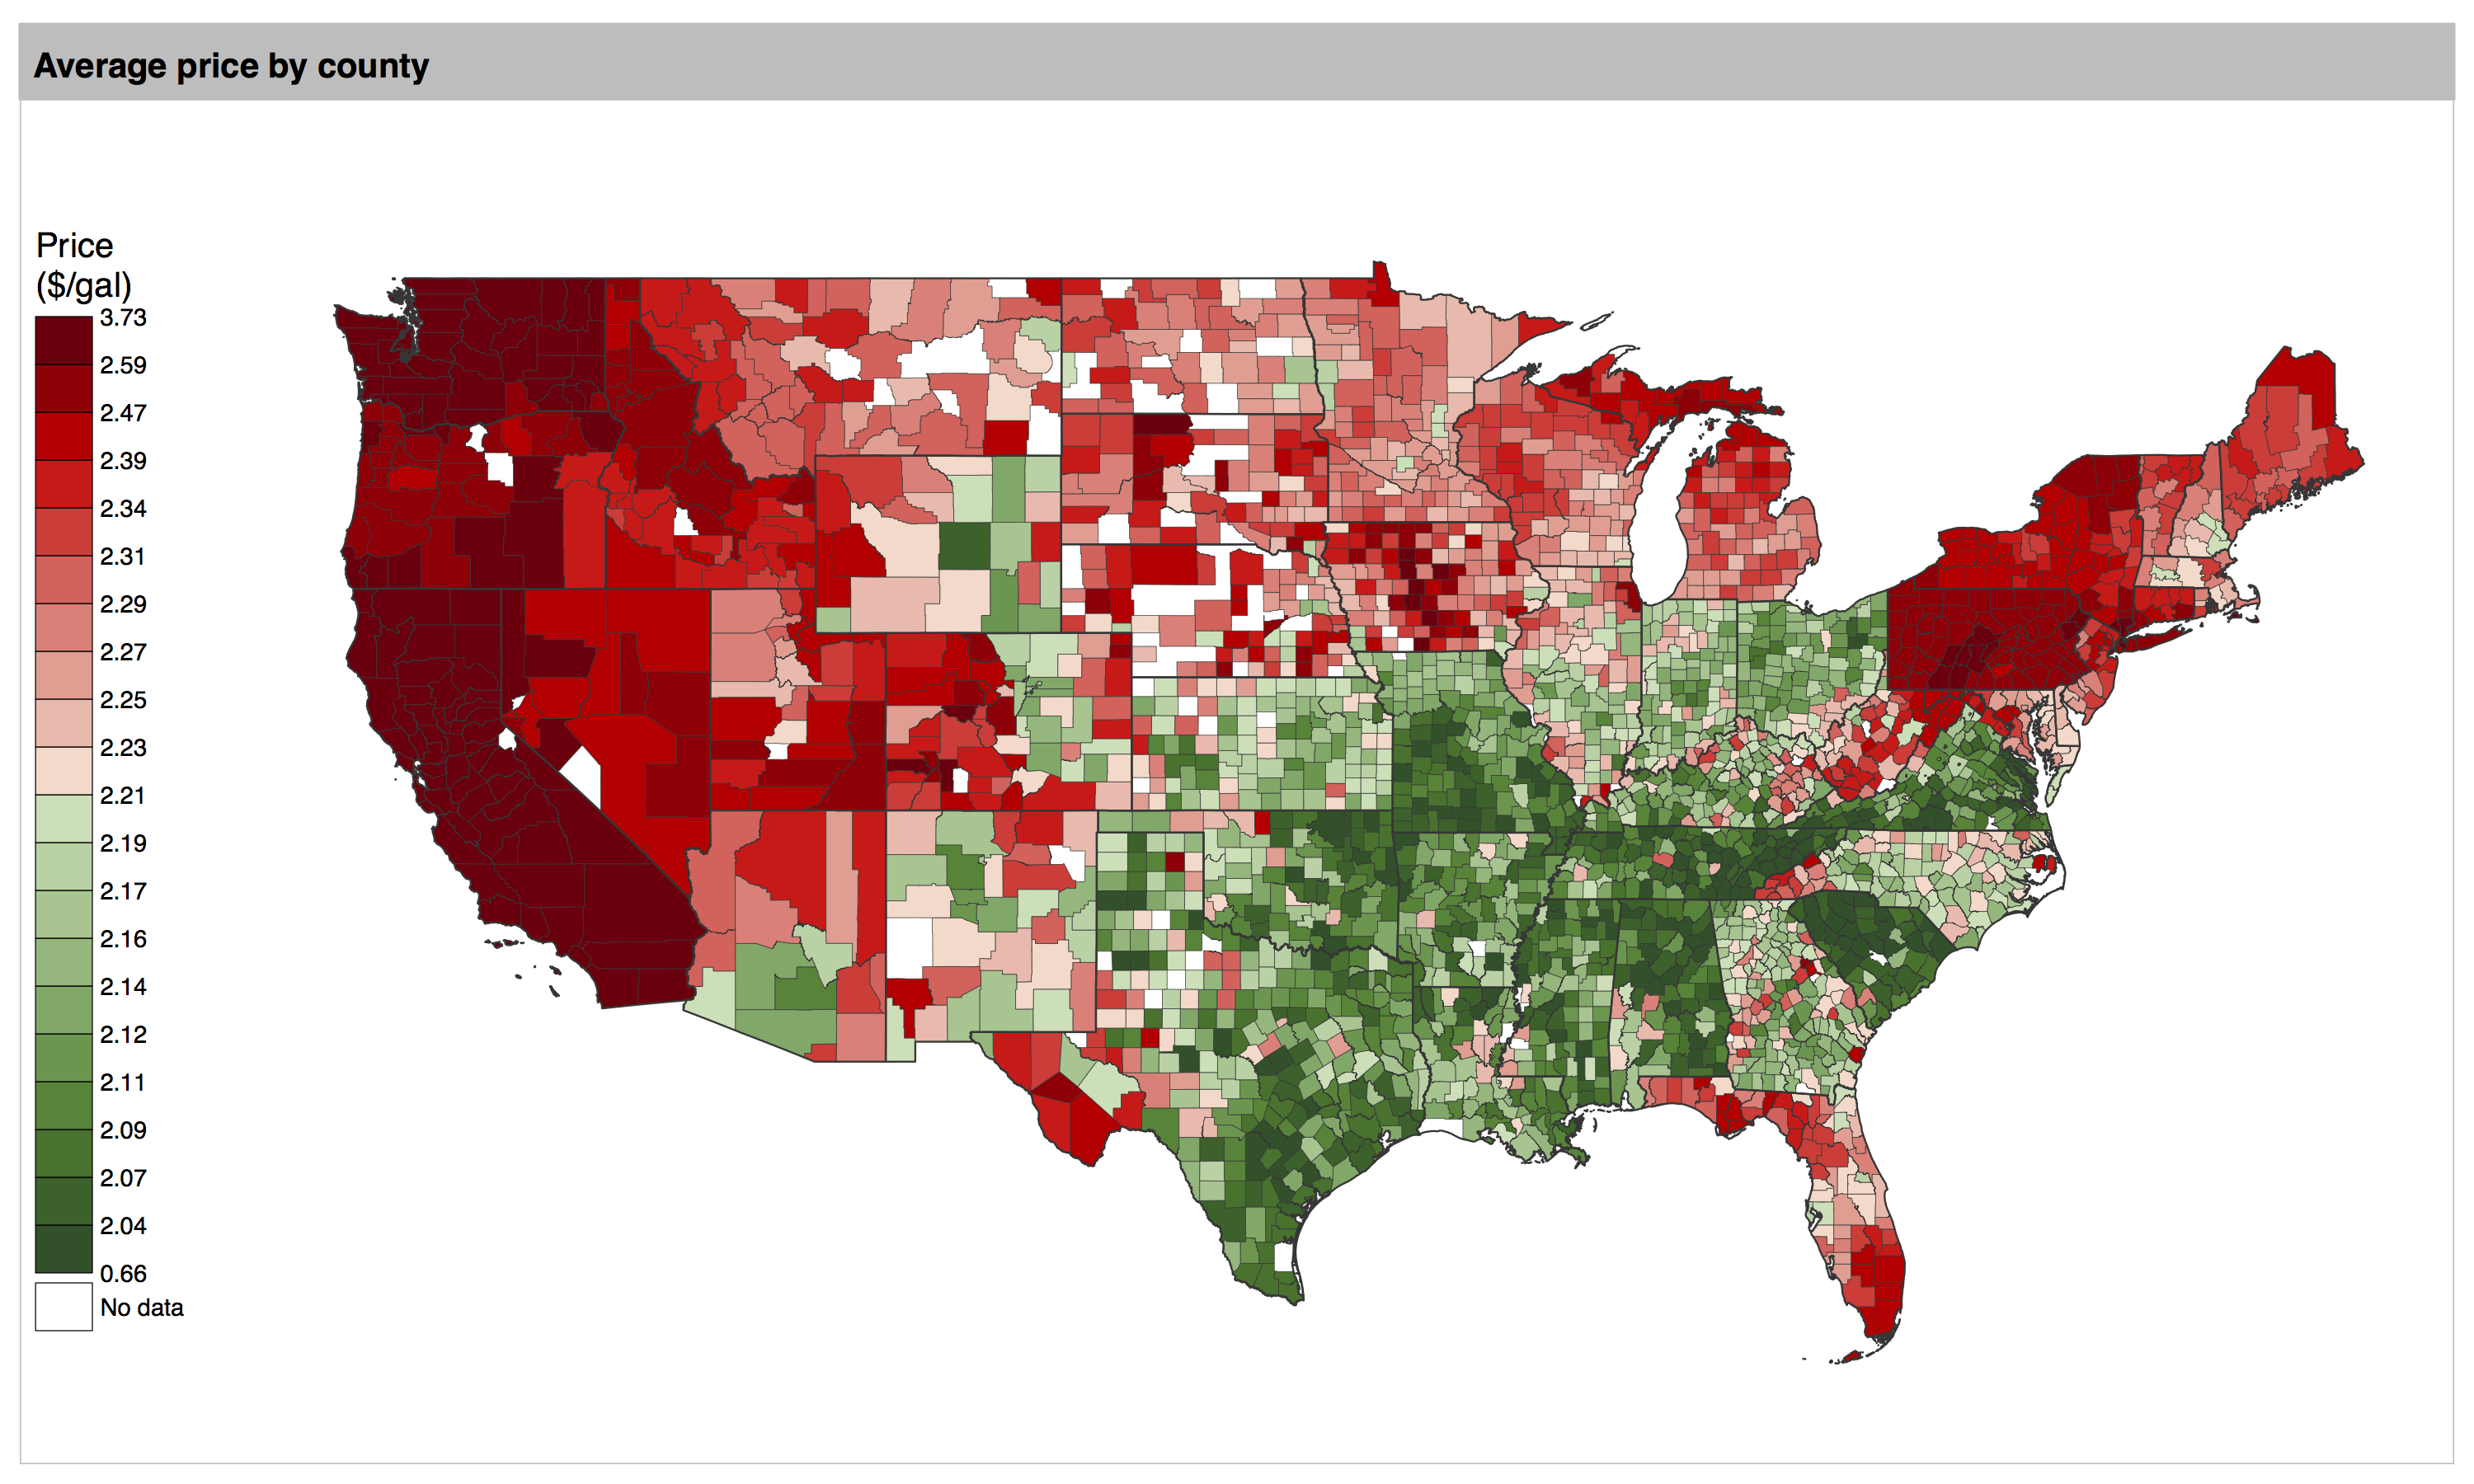
\includegraphics[width=\textwidth]{average_regular_map}
\caption{Map of mean price for counties, regular fuel, averaged over the whole period.}\vspace{-0.3cm}
\label{fig:map_price}
\end{figure}

Since most of the variation in oil price is between gas station, we now focus mainly on spatial correlations. We will conduct the analysis at the county level for various reasons. First it appears that a variance decomposition of fuel price between and within county shows that more than 85\% of the variance is between-county, second because the localization of gas station is not reliable enough to allow for a smaller granularity and third because we have many socio-economic information at this level. We therefore study the spatial autocorrelation of prices at the county level. Spatial autocorrelation can be seen as an indicator of spatial heterogeneity which we measure using the Moran index~(\cite{tsai2005quantifying}), with spatial weights of the form $\exp{\left(-d_{ij} / d_0 \right)}$ with $d_{ij}$ being the distance between spatial entities $i$ and $j$, and $d_0$ a decay parameter giving the spatial range of interactions accounted for in the computation. We show in Fig.~\ref{fig:moran} its variations for each day and also as a function of the decay parameter. 
The fluctuations in time of the daily Moran index for low and medium spatial range, confirms geographical specificities in the sense of locally changing correlation regimes. These are logically smoothed for long ranges, as price correlations drop down with distance. The behavior of spatial autocorrelation with decay distance is particularly interesting: we observe a first regime change around 10km (from constant to piecewise linear regime), and a second important one around 1000km, both consistent across weekly time windows. We postulate that these correspond to typical spatial scales of the involved processes: the low regime would be local specificities and the middle one the state level processes. This behavior confirms that prices are non-stationary in space, and that therefore appropriate statistical techniques must be used to study potential drivers at different level. The two next subsections follow this idea and investigate potential explicative variables of local fuel prices, using two different techniques corresponding to two complementary paradigms: geographically weighted regression that puts the emphasis on neighborhood effects, and multi-level regression taking into account administrative boundaries.

\begin{figure}
\centering
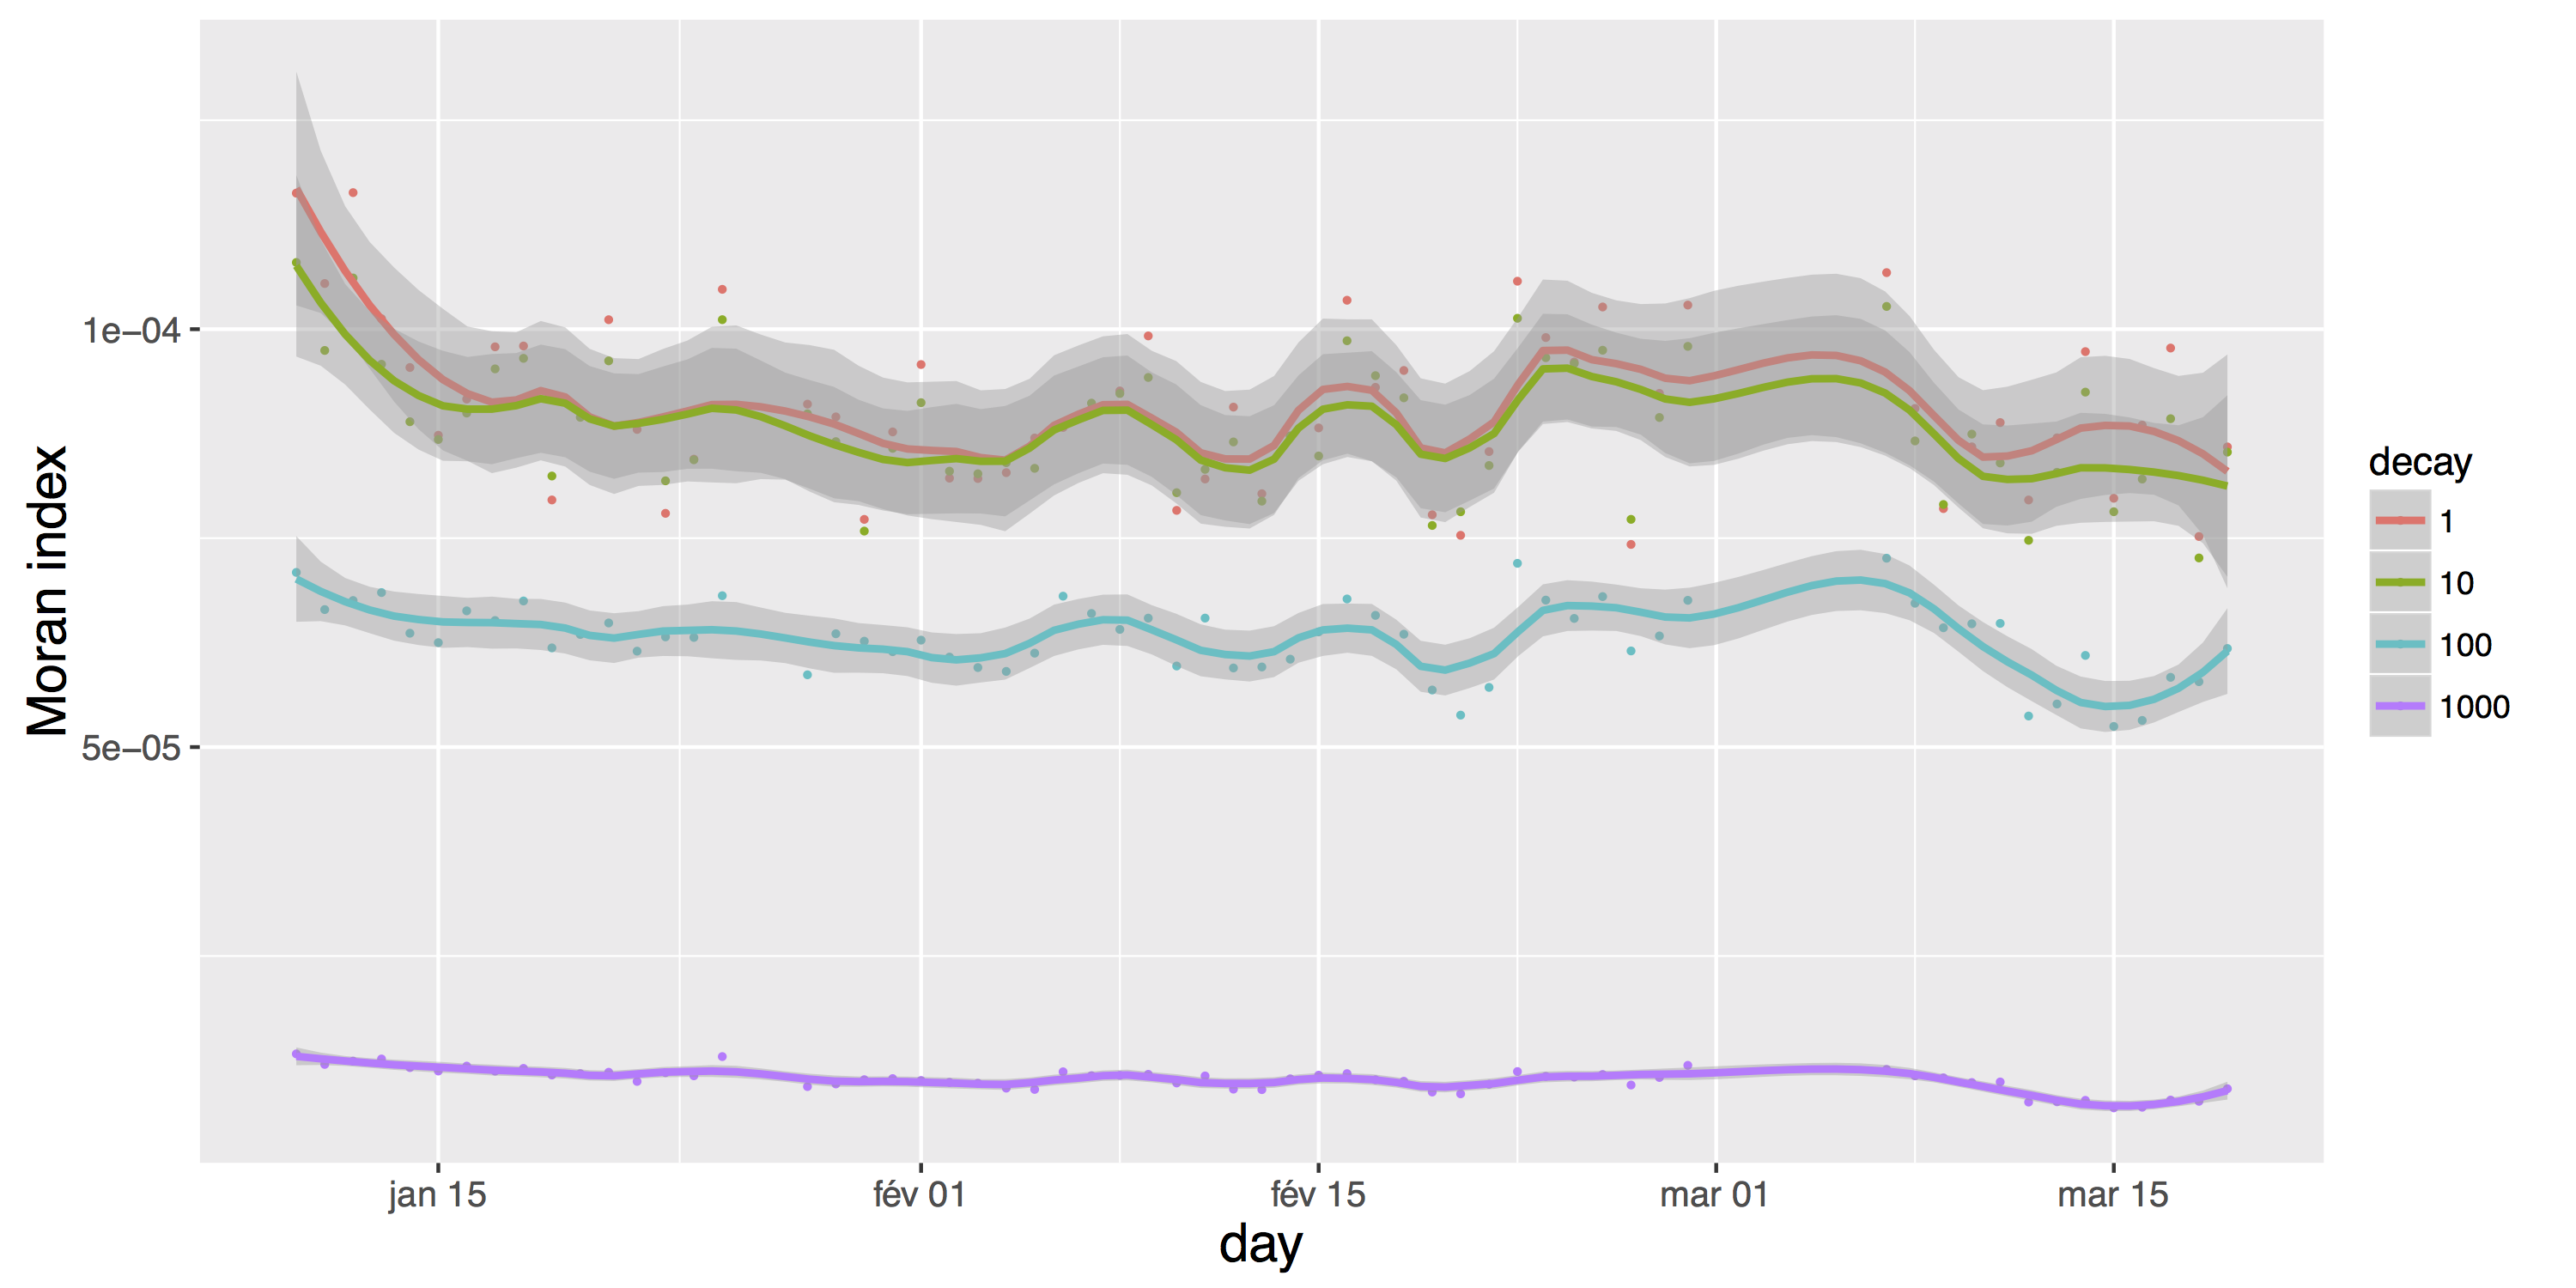
\includegraphics[width=0.48\textwidth]{moran_days}
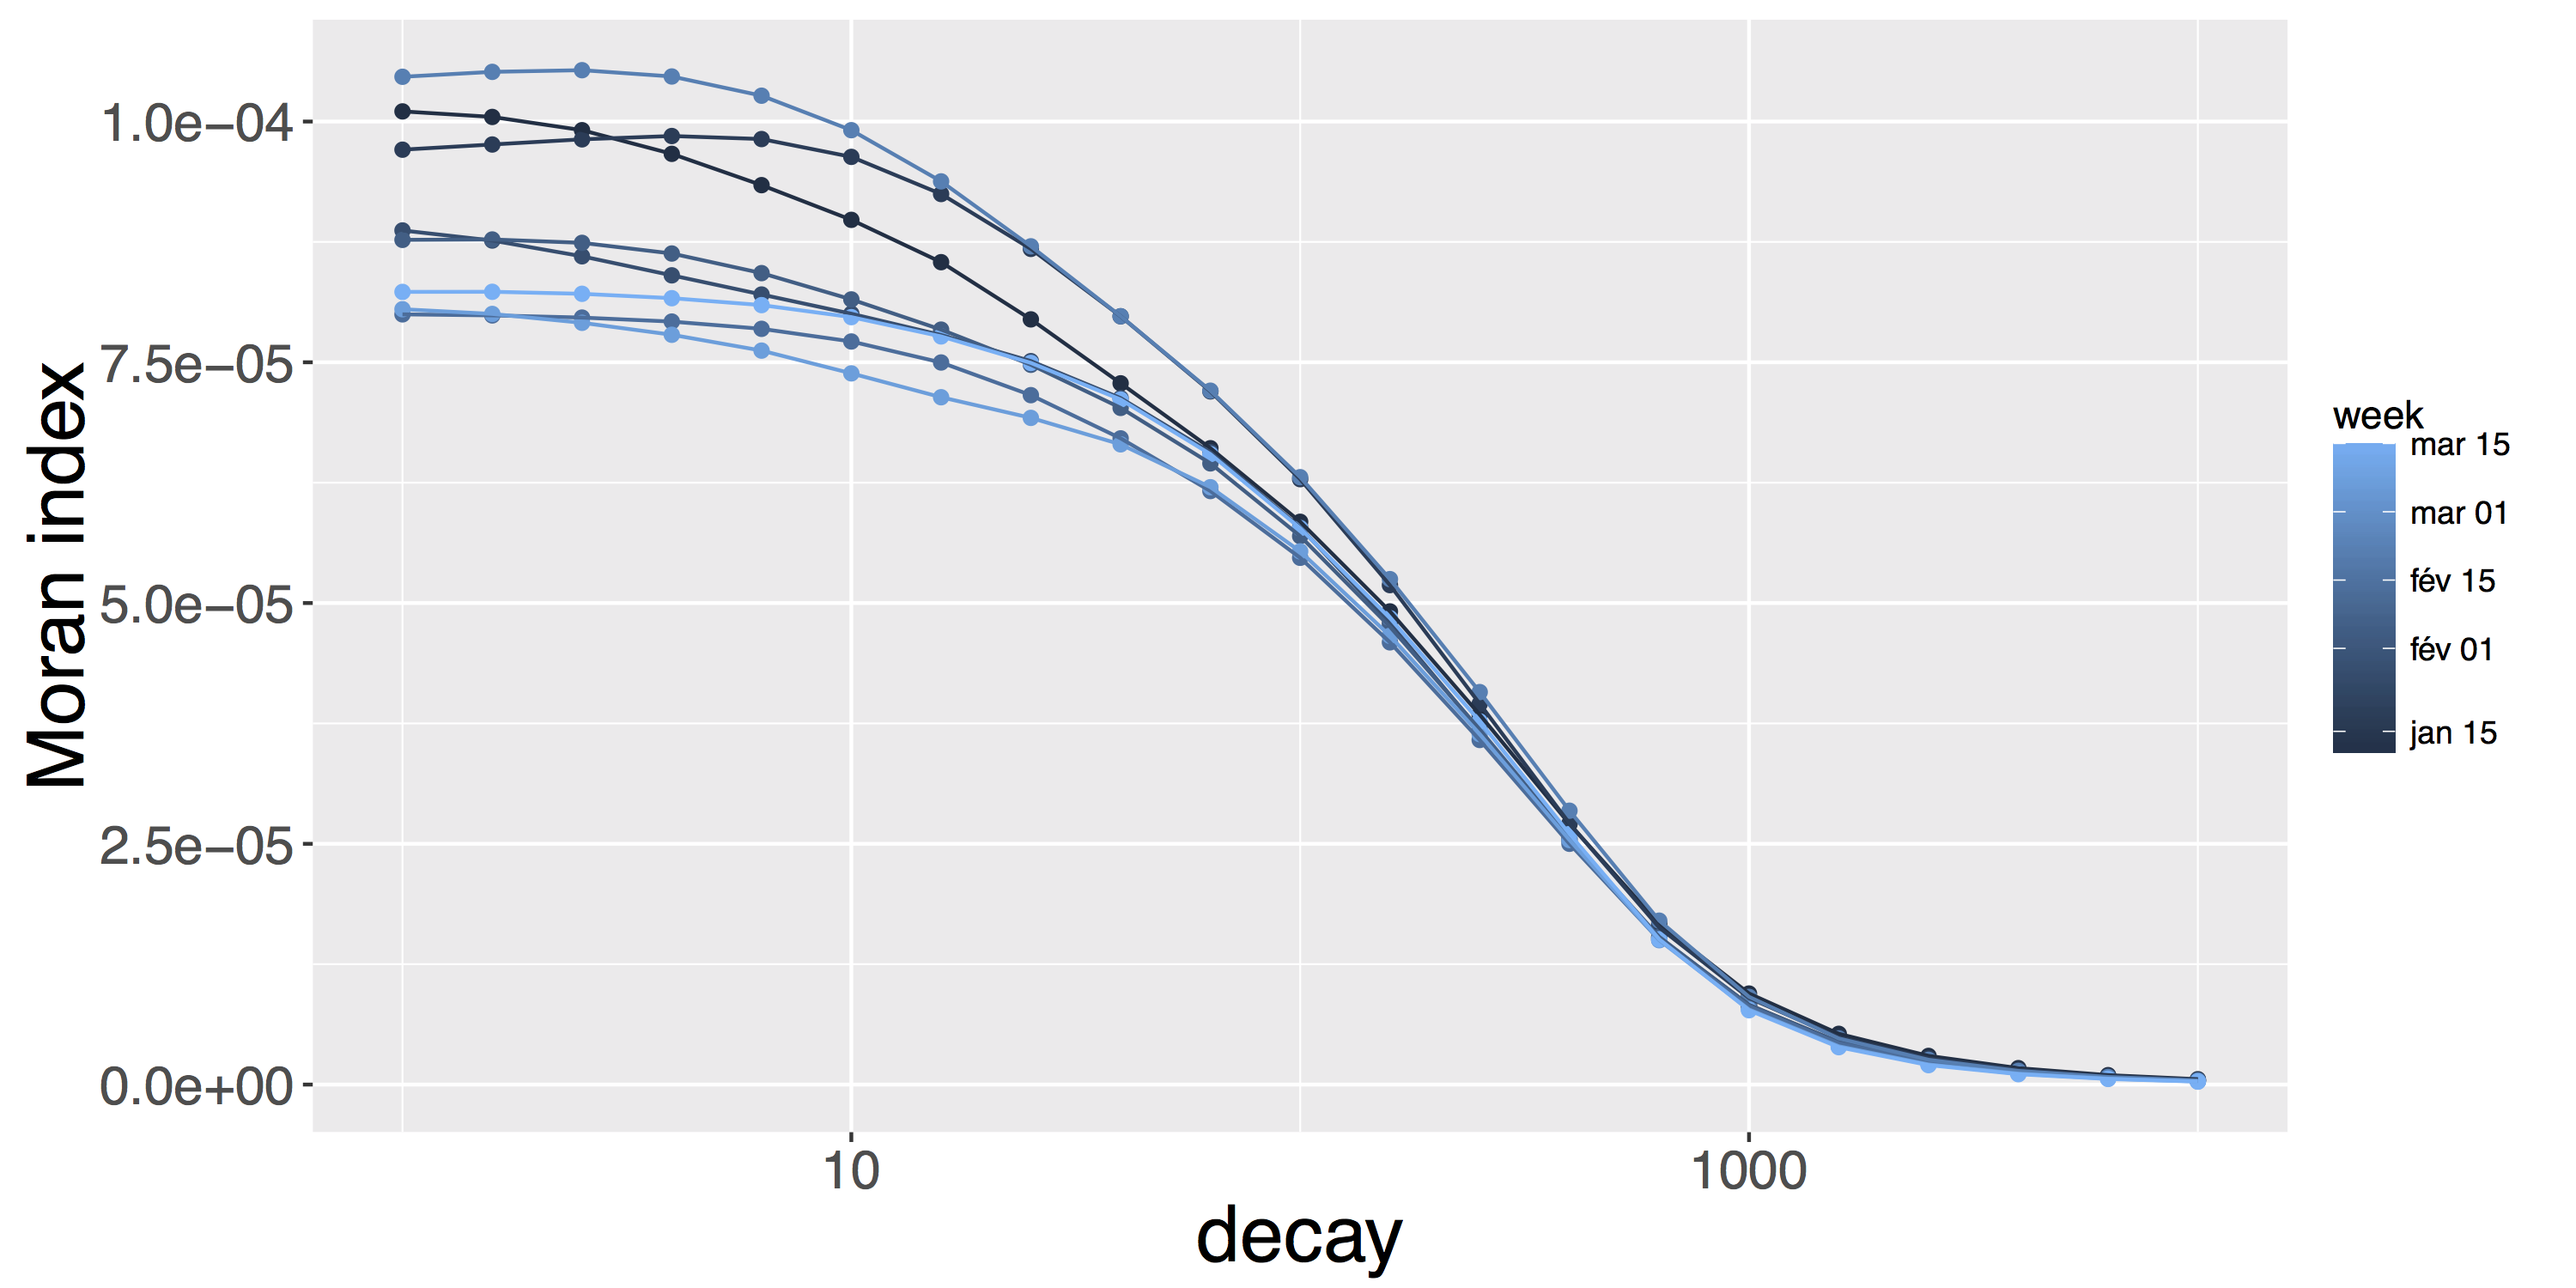
\includegraphics[width=0.48\textwidth]{moran_decay_weeks}
\caption{\textbf{Behavior of Moran spatial-autocorrelation index.} (Left) Evolution in time of Moran index computed on daily time windows, for different decay parameter values. (Right) Moran index as a function of decay parameter, computed on weekly time windows.}
\label{fig:moran}
\end{figure}

\subsection{Geographically Weighted Regression}

The issue of spatial non-stationarity of geographical processes has always been a source of biased aggregated analyses or misinterpretations when applying general conclusions to local cases. To take it into account into statistical models, numerous techniques have been developed, among which the simple but very elegant Geographically Weighted Regression (GWR), that estimates non-stationary regressions by weighting observations in space similarly to kernel estimation methods. This was introduced in a seminal paper by~\cite{brunsdon1996geographically} and has been subsequently used and matured since then. The significant advantage of this technique is that an optimal spatial range in the sense of model performance can be inferred to derive a model that yields the effect of variables varying in space, thus revealing local effects that can occur at different spatial scales or across boundaries. We proceed to multi-modeling to find the best model and associated kernel and spatial range. More specifically, we do the following: (i) we generate all possible linear models from the five potential variables (income, population, wage per job, jobs per capita, jobs); (ii) for each model and each candidate kernel shape (exponential, gaussian, bisquare, step), we determine the optimal bandwidth in the sense of both cross-validation and corrected Akaike Information Criterion (AICc) which quantifies information included in the model; (iii) we fit the models with this bandwidth. We choose the model with the best overall AICc, namely $price = \beta\cdot\left( income, wage, percapjobs\right)$ for a bandwidth of 22 neighbors and a gaussian kernel,\footnote{note that the kernel shape does not have much influence as soon as gradually decaying functions are used} with an AICc of $2,900$. The median AICc difference with all other models tested is 122. The global R-squared is 0.27, what is relatively good also compared to the best R-squared of 0.29 (obtained for the model with all variables, which clearly overfits with an AICc of 3010; furthermore, effective dimension is less than 5 as 90\% of variance is explained by the three first principal components for the normalized variables).

The coefficients and local R-squared for the best model are shown in Fig.~\ref{fig:gwr}. The spatial distribution of residuals (not shown here) seems globally randomly distributed, which confirms in a way the consistency of the approach. Indeed, if a distinguishable geographical structure had been found in the residuals, it would have meant that the geographical model or the variable considered had failed to translate spatial structure. Let now turn to an interpretation of the spatial structures we obtain. First of all, the spatial distribution of the model performance reveals that regions where these simple socio-economic factors explain do a good job in explaining prices are mostly located on the west coast, the south border, the north-east region from lakes to the east coast, and a stripe from Chicago to the south of Texas. The corresponding coefficients have different behaviors across the areas, suggesting different regimes.\footnote{We comment their behavior in areas where the model has a minimal performance, that we fix arbitrarily as a local R-squared of 0.5} For example, the influence of income in each region seems to be inverted when the distance to the coast increases (from north to south-east in the west, south to north in Texas, east to west in the east), what may be a fingerprint of different economic specializations. On the contrary, the regime shifts for wage show a clear cut between west (except around Seattle) and middle/east, that does not correspond to state-policies only as Texas splits in two. The same way, jobs per capita show an opposition between east and west, what could be due for example to cultural differences. These results are difficult to interpret directly, and must be understood as a confirmation that geographical particularities matters, as regions differ in regimes of role for each of the simple socio-economic-variables. Further precise knowledge could be obtained through targeted geographical studies including qualitative field studies and quantitative analyses, that are beyond the scope of this exploratory paper and left for further research.

Finally, we extract the spatial scale of the studied processes, that is, by computing the distribution of distance to nearest neighbors with the optimal bandwidth. It yields roughly a log-normal distribution, of median 77km and interquartile 30km. We interpret this scale as the spatial stationarity scale of price processes in relation with economic agents, which can also be understood as a range of coherent market competition between gas stations.

\begin{figure}
\centering
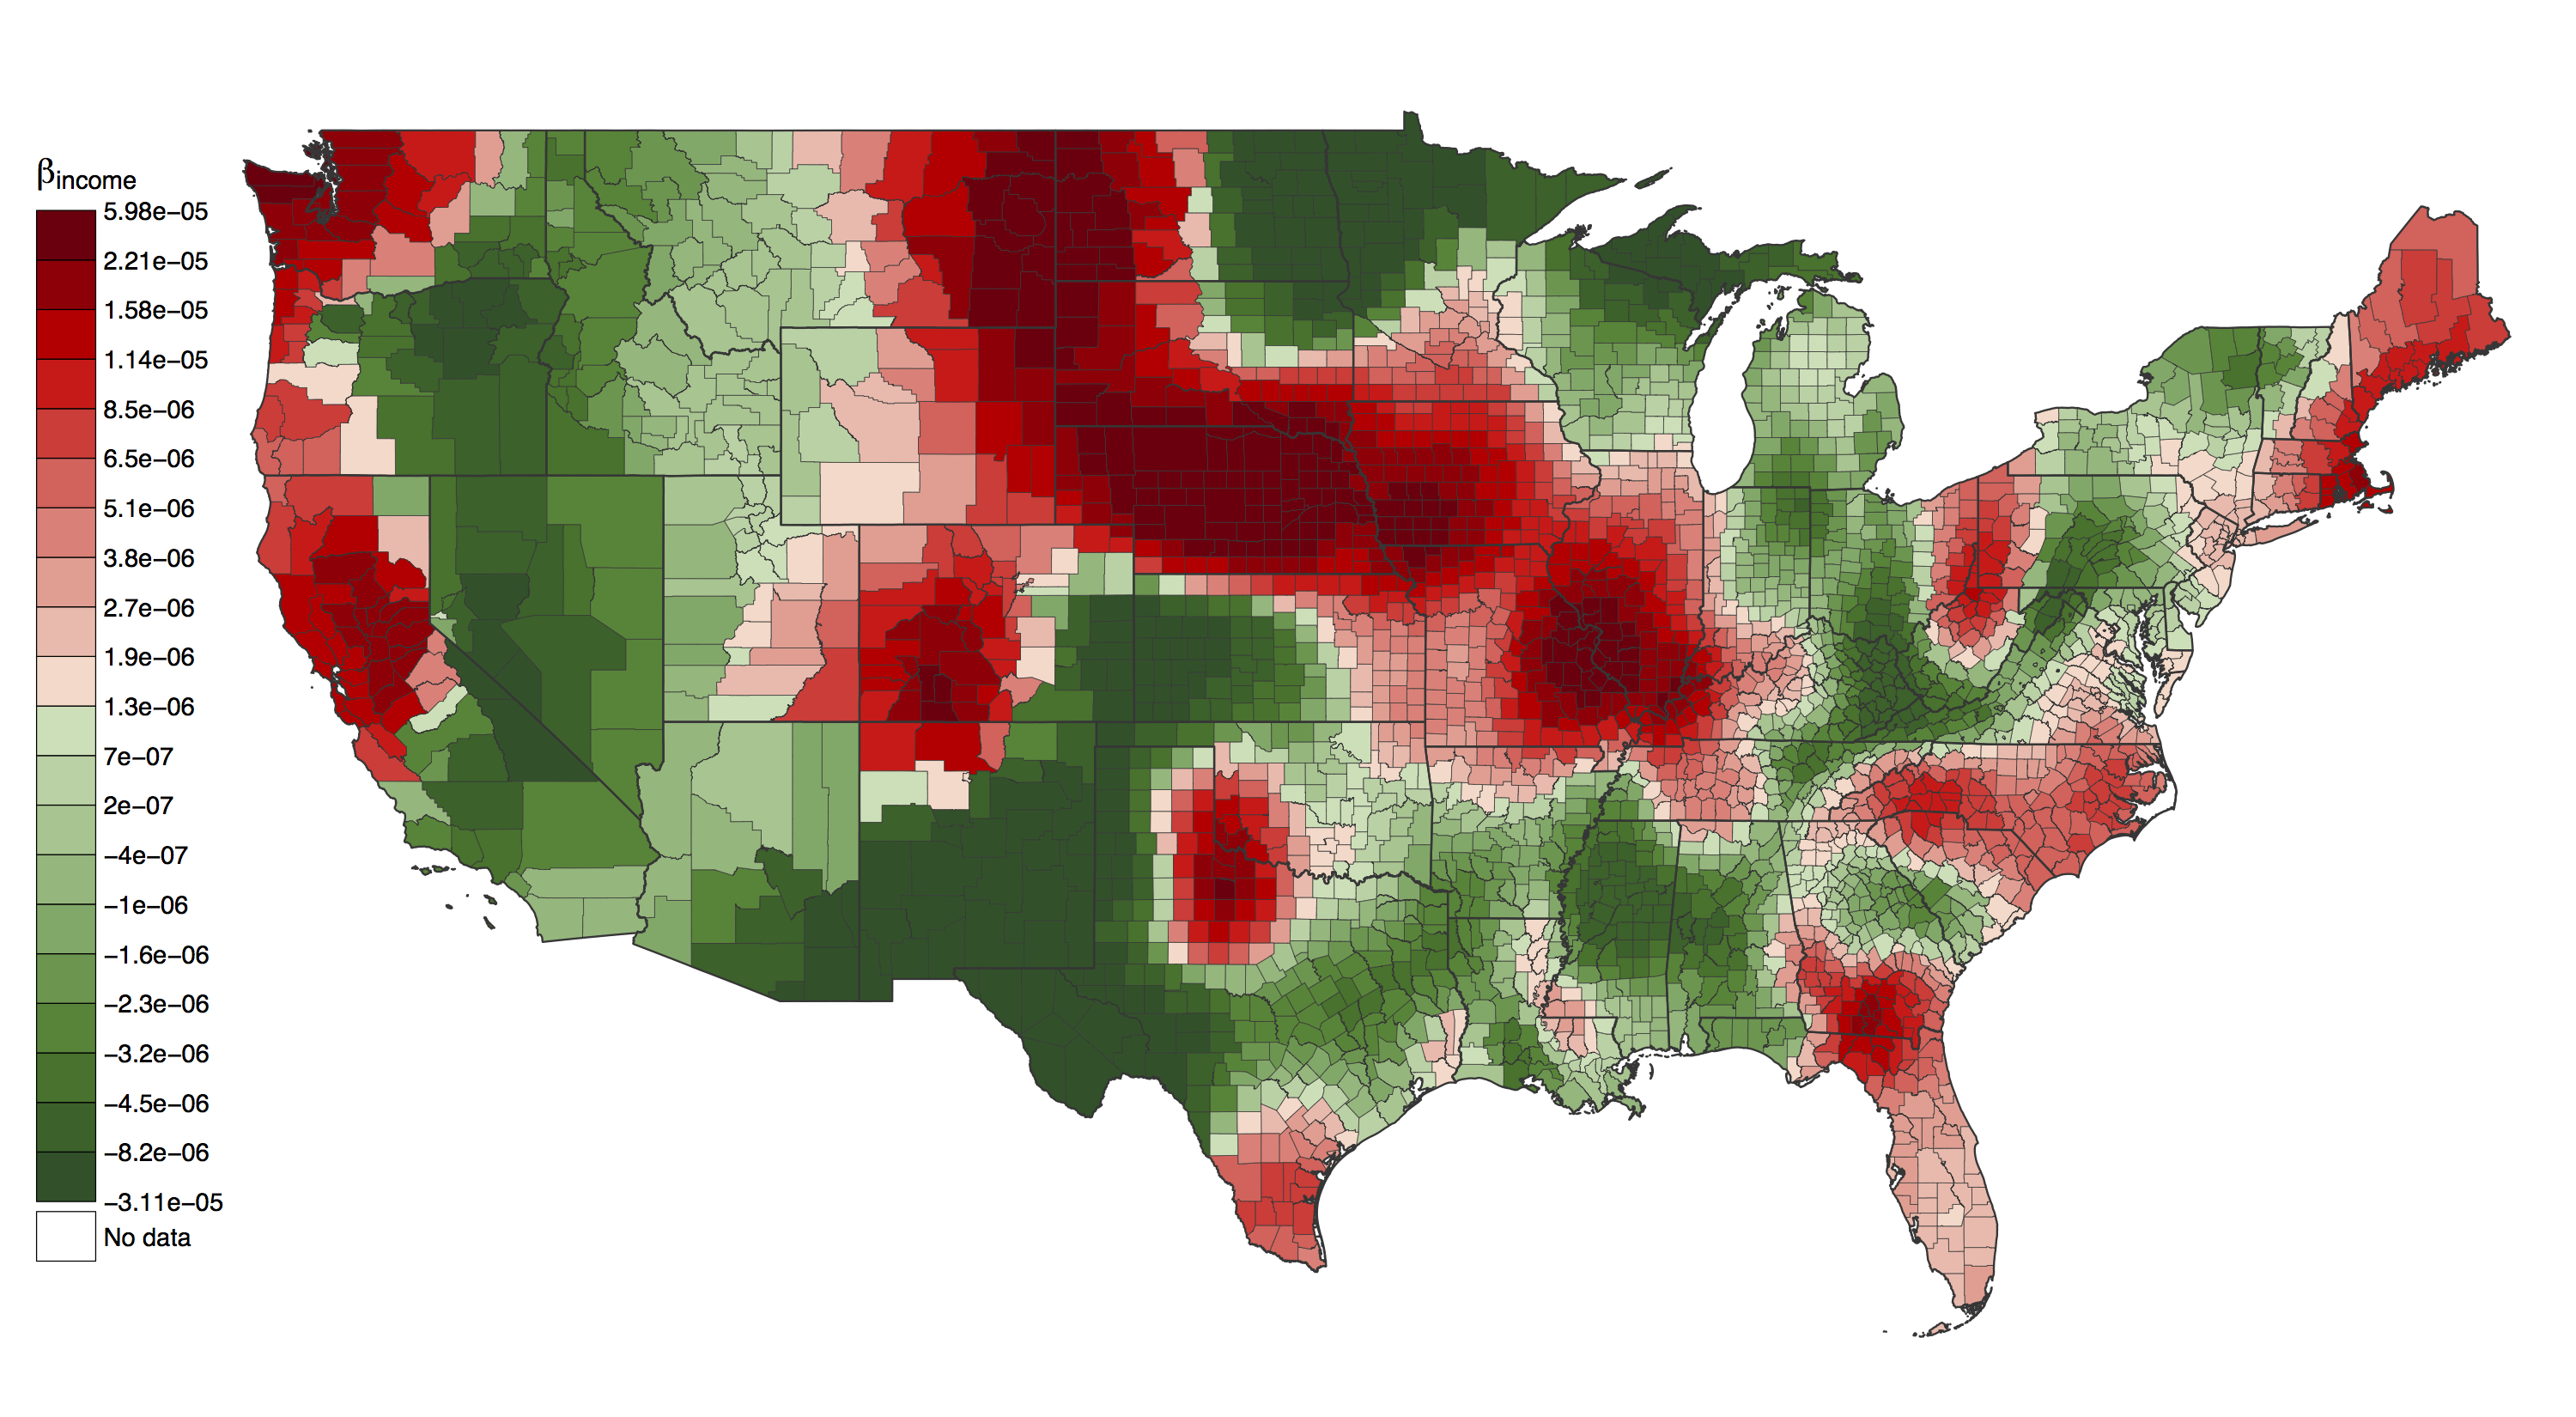
\includegraphics[width=0.48\textwidth]{gwr_allbest_betaincome}
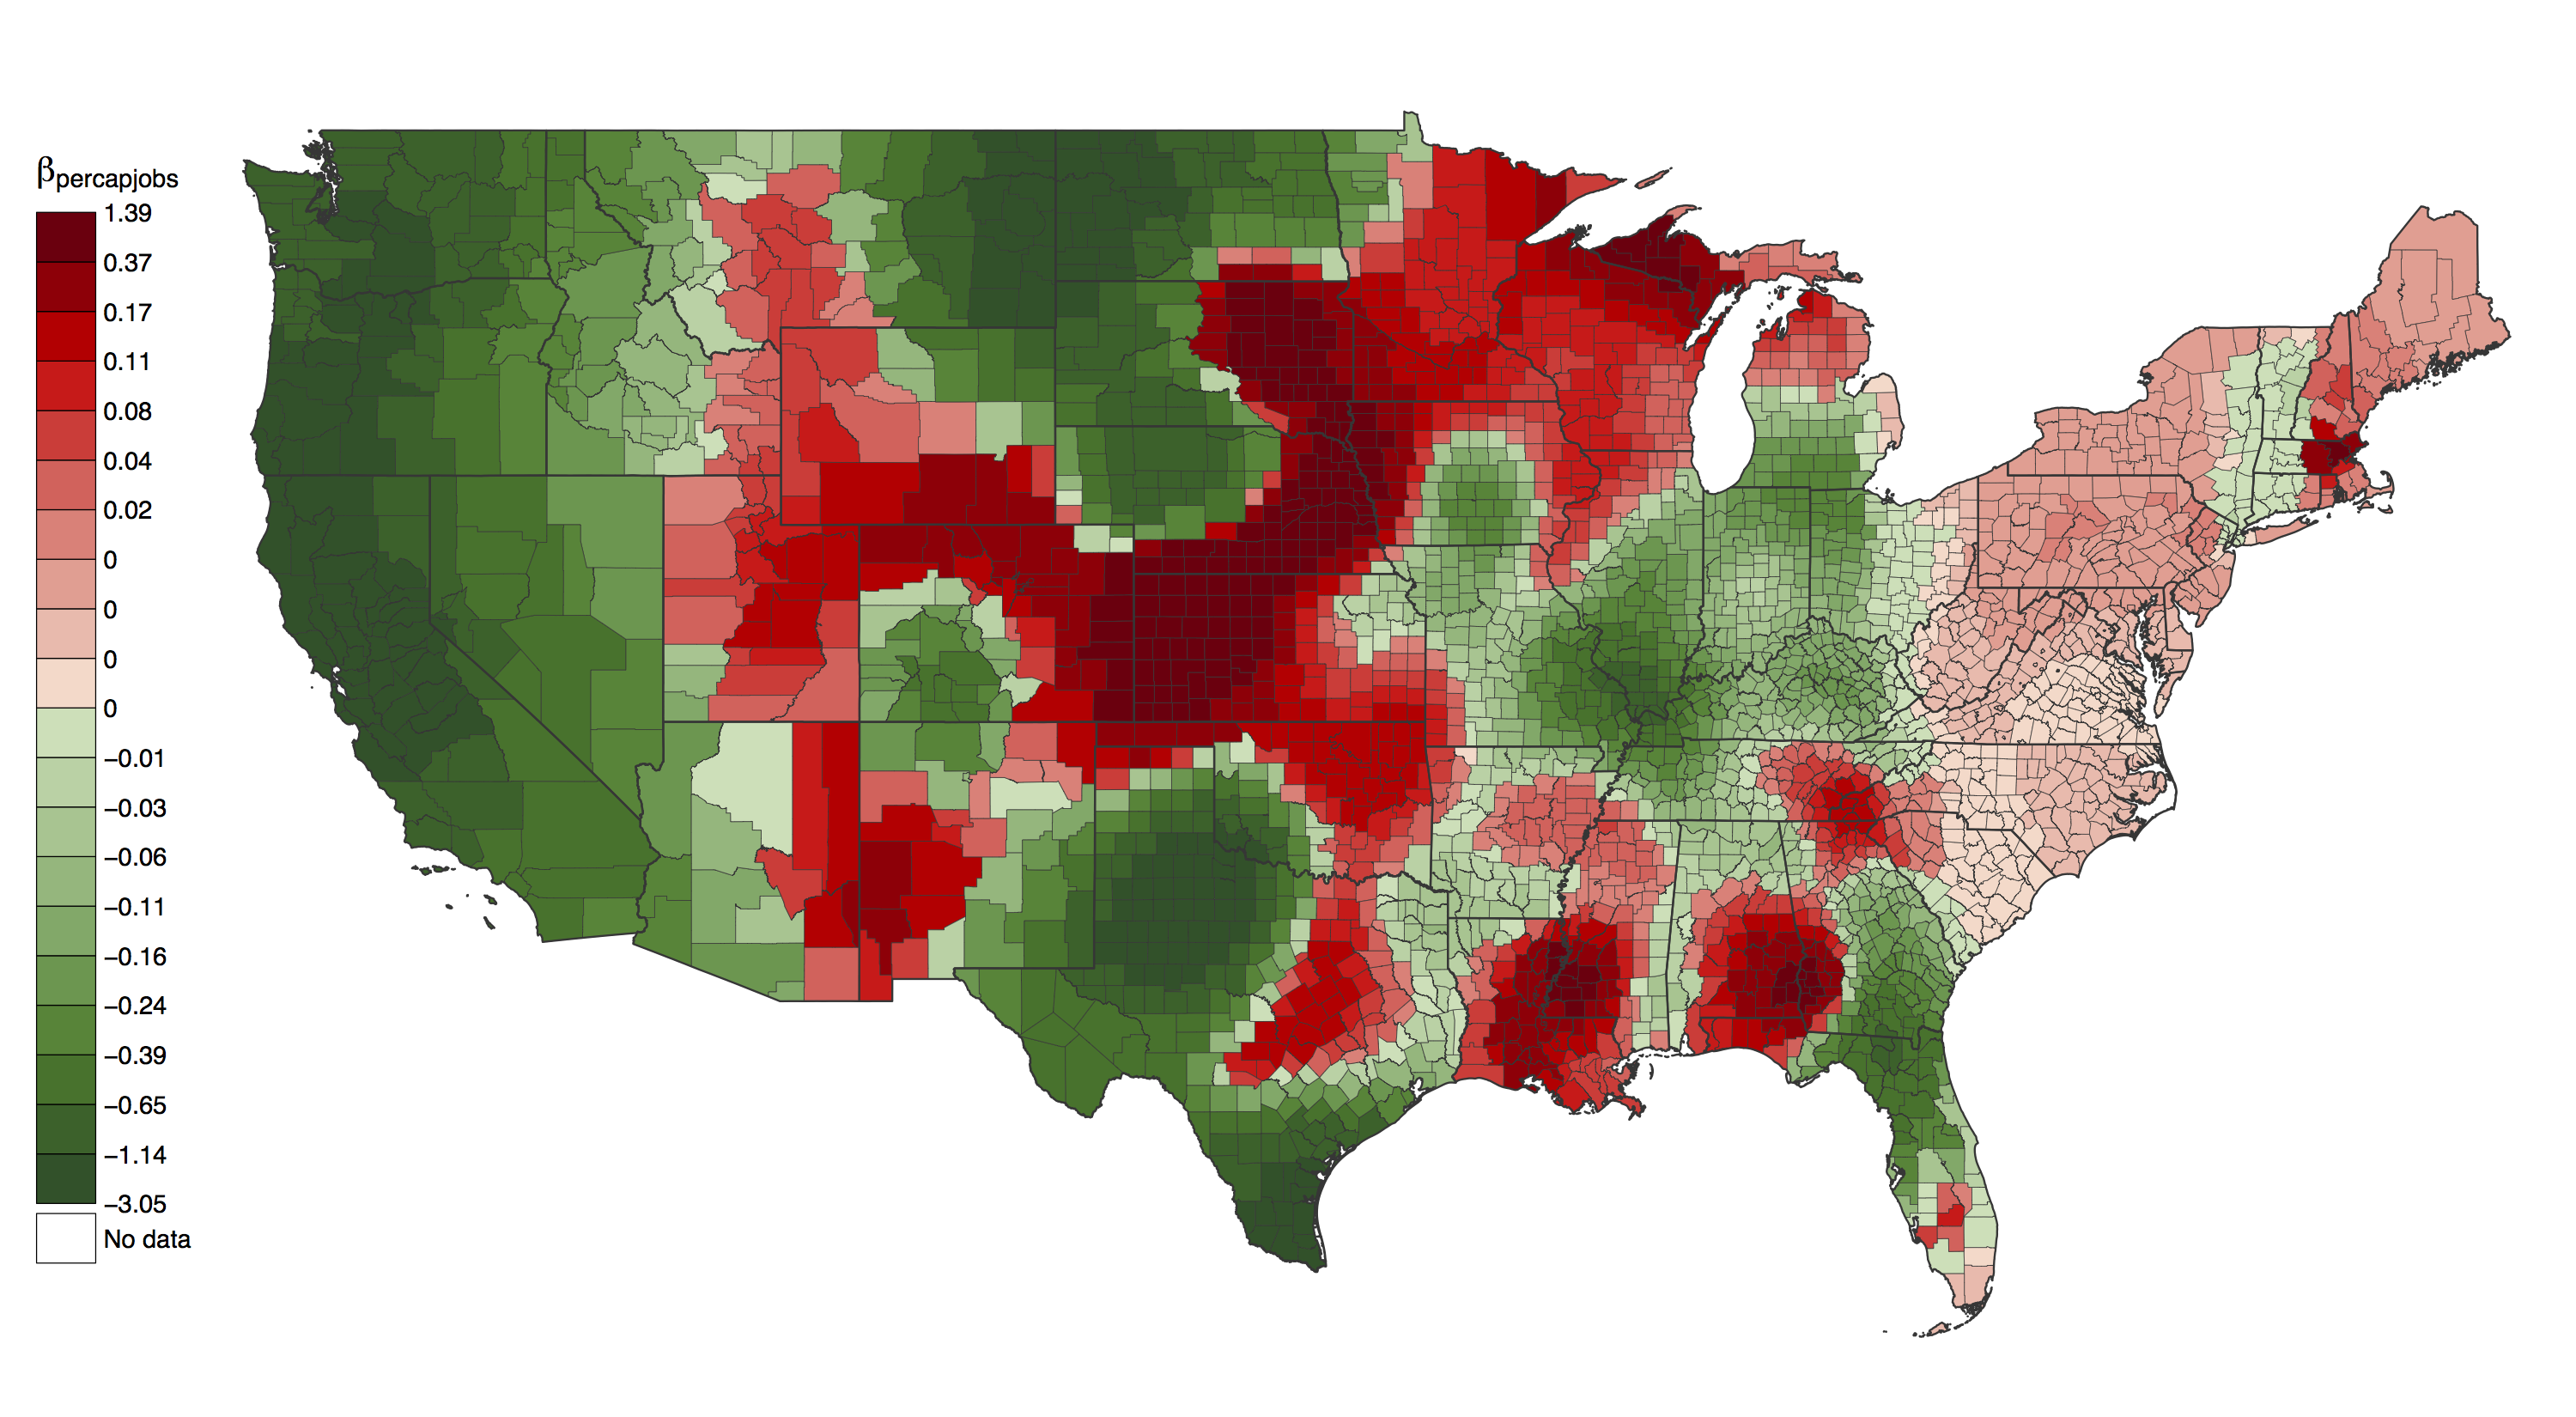
\includegraphics[width=0.48\textwidth]{gwr_allbest_betapercapjobs}\\
%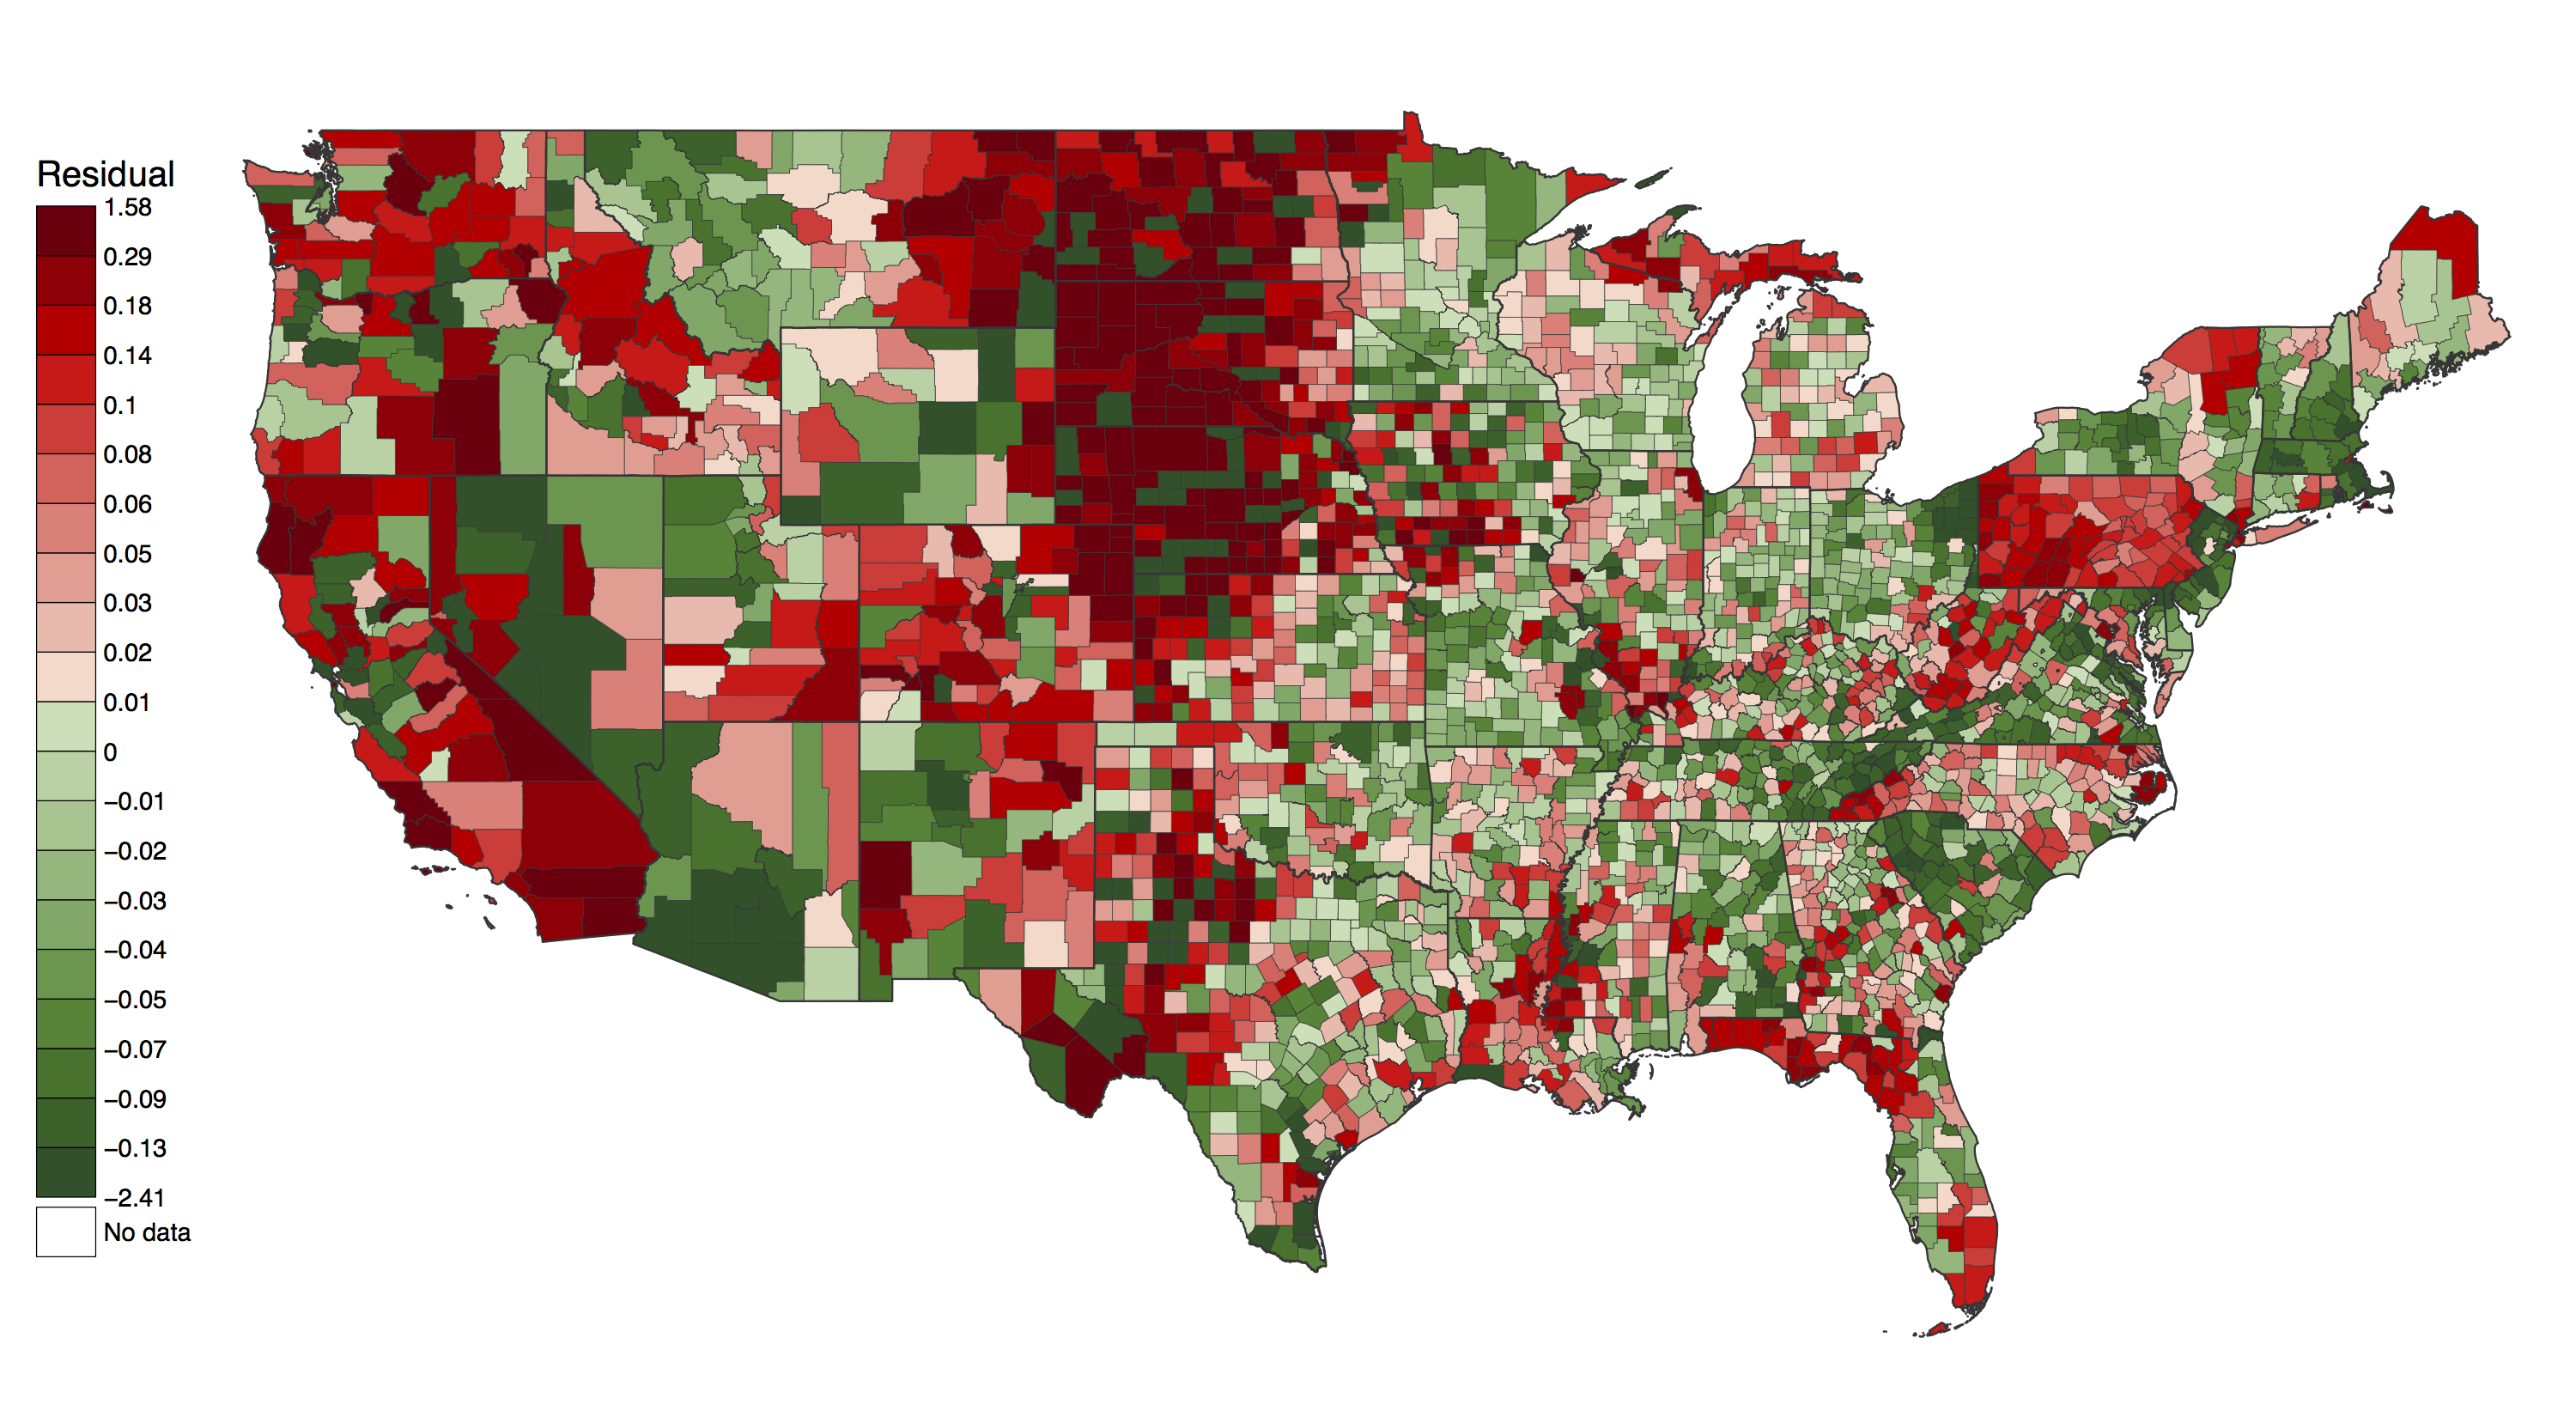
\includegraphics[width=0.48\textwidth]{figures/gwr_allbest_residual}
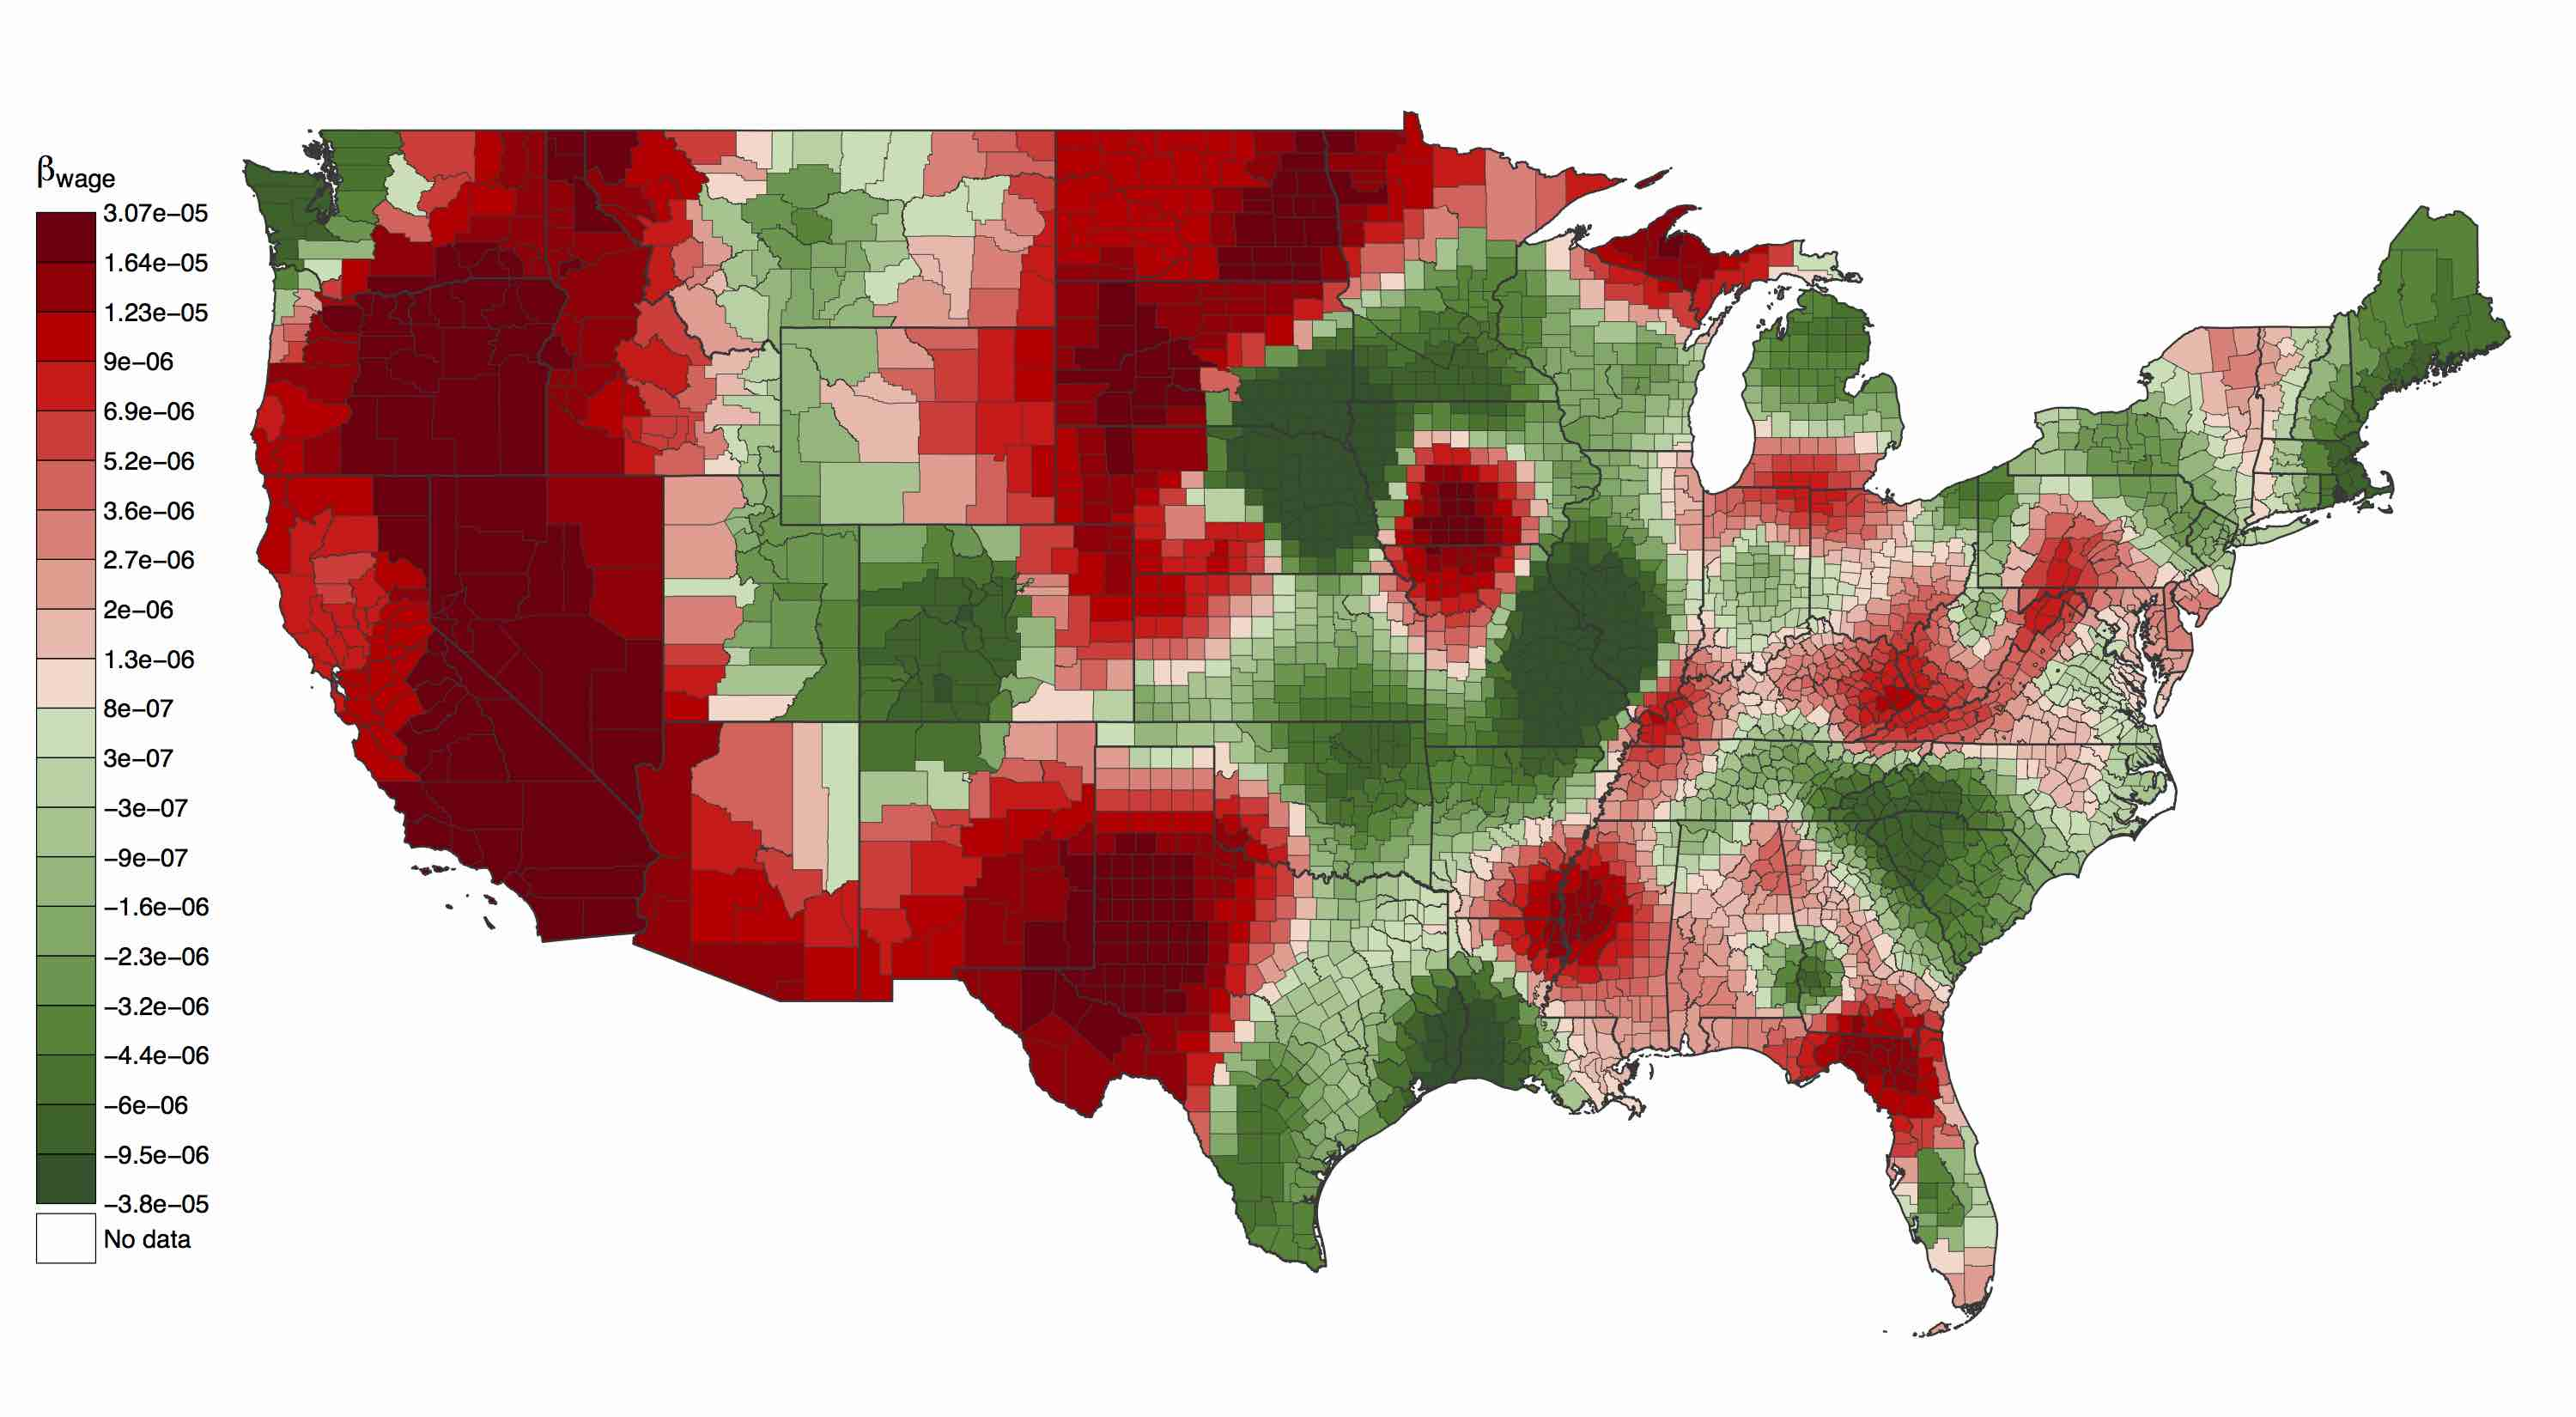
\includegraphics[width=0.48\textwidth]{gwr_allbest_wage}
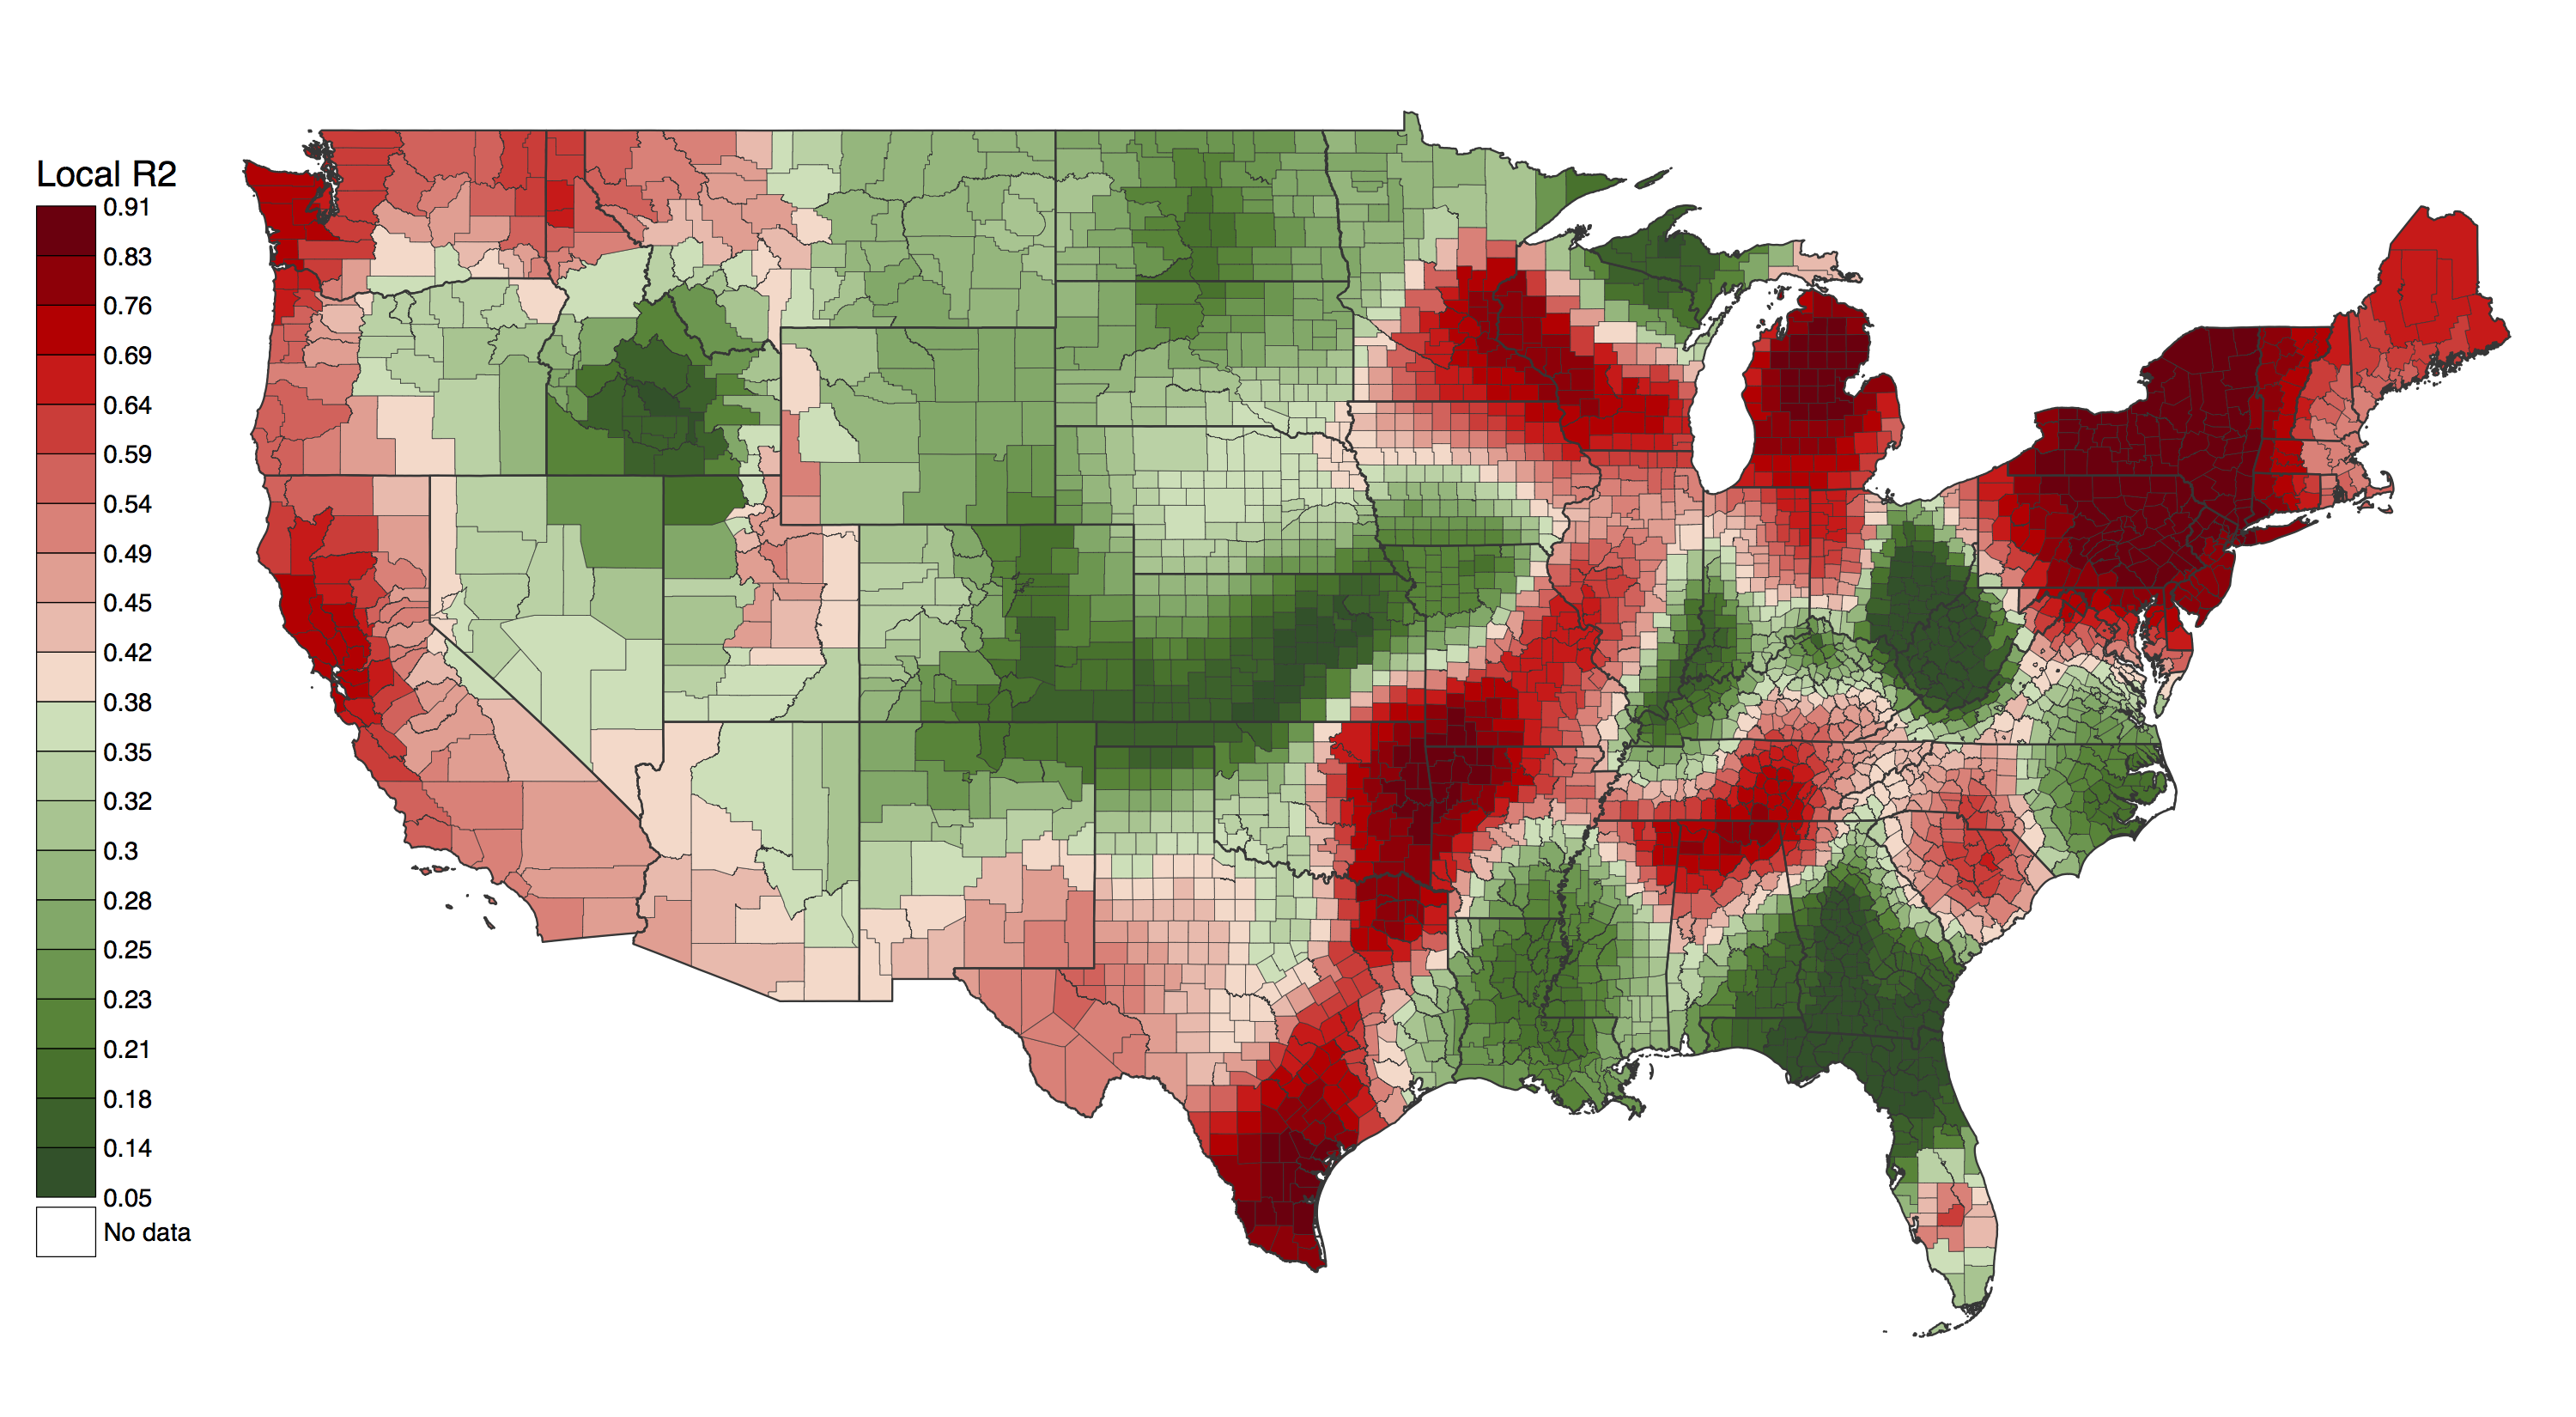
\includegraphics[width=0.48\textwidth]{gwr_allbest_LocalR2}
\caption{\textbf{Results of GWR analyses.} For the best model in the sense of AICc, we map the spatial distribution of fitted coefficient, in order from left to right and top to bottom, $\beta_{income}$, $\beta_{percapjobs}$, $\beta_{wage}$, and finally the local r-squared values.}
\label{fig:gwr}
\end{figure}

\subsection{Multi-level Regression}

Since our initial database enables to look at the level of variable $x_{i,s,c,t}$, the fuel price in day $t$, in gas station $i$, in state $s$ and in county $c$, we start by running high dimensional fixed effect regressions following the model:
\begin{eqnarray}
x_{i,s,c,t} &=& \beta_s + \varepsilon_{i,s,c,t} \\
x_{i,s,c,t} &=& \beta_c + \varepsilon_{i,s,c,t} \\
x_{i,s,c,t} &=& \beta_i + \varepsilon_{i,s,c,t}\\
\end{eqnarray}

Where $\varepsilon_{i,s,c,t}$ contains an idiosyncratic error and a day fixed effect. This first analysis confirm that most of the variance can be explained by a state fixed effect and that integrating more accurate levels has only small effect on the fit of our model as measured by the R-squared.

We now turn to a different analysis, aiming at capturing the explanatory variables that account for spatial price variation of fuel. We consider the following linear model:

\begin{equation}
\label{eq:reg}
log(x_{i}) = \beta_0 + X_{i}\beta_1 + \beta_{s(i)} + \varepsilon_{i},
\end{equation}

where $x_{i}$ denotes average measured fuel price in county $i$ aggregated across all days, $X_{i}$ is a set of county specific variables and $s(i)$ is the state to which the county belongs so that $\beta_{s(i)}$ capture all state specific variation. Finally $\varepsilon_{i}$ is an error term satisfying $Cov(\varepsilon_{i}, \varepsilon_{j}) = 0$ if $s(i) \neq s(j)$. This clustering of standard error at the state level is motivated by finding of the previous section, showing that spatial autocorrelation of fuel price at the state level is still potentially strong. This specification aims at capturing the effect of various socio-economic variable at the county level after a state fixed effect has been removed. We present our results in Table~\ref{tab:reg}. Column (1) shows that regressing the log of price on a state fixed-effect is already enough to explain 74\% of the variance. This is mostly due to tax on fuel which are set at the state level in the US. In fact, when we regress the log of oil price on the level of state tax, we find a R-squared of 0.33\%. The remaining explanatory variables show that dense urban counties have higher fuel price, but this price decreases with population. This result seems sensible, desert areas have on average higher oil price. Fuel price increases with total income, decreases with poverty and decrease with the extent to which a county has voted for a Republican candidate. This last finding suggests a circular link: counties that use car the most tend to vote to politician that promote pro car policies.
Adding these explanatory variables slightly increase the R-squared, suggesting that even after having removed a state fixed-effect, the price of fuel can be explained by local socio-economic features.	

\begin{table}[htbp]
\vspace{-0.1cm}
\begin{center}
{
\begin{threeparttable}
\caption{\footnotesize{\textsc{Regressions at the county level}}}
\label{tab:reg}
\begin{tabular}{lccccc}
 \toprule
 \hline
 \cr

  & (1) & (2) & (3) & (4) & (5) \\ 
\cmidrule(r){2-6}
Density      &               &       0.016***&       0.016***&       0.016***&       0.015***\\
                    &               &     (0.002)   &     (0.001)   &     (0.001)   &     (0.001)   \\ \cr
Population (log)             &               &      -0.007***&      -0.040***&      -0.041***&      -0.039***\\                    &               &     (0.001)   &     (0.011)   &     (0.011)   &     (0.010)   \\ \cr
Total Income (log)            &               &               &       0.031***&       0.031***&       0.027***\\
                    &               &               &     (0.010)   &     (0.010)   &     (0.009)   \\ \cr
Unemployment        &               &               &       0.001   &       0.000   &       0.000   \\
                    &               &               &     (0.001)   &     (0.001)   &     (0.001)   \\ \cr
Poverty   &               &               &      -0.028** &      -0.030***&      -0.029** \\
                    &               &               &     (0.011)   &     (0.011)   &     (0.011)   \\ \cr
Percentage Black    &               &               &               &       0.000***&      -0.000   \\
                    &               &               &               &     (0.000)   &     (0.000)   \\ \cr
Vote GOP      &               &               &               &               &      -0.072***\\
                    &               &               &               &               &     (0.015)   \\ \cr 
\cmidrule{2-6}
R-squared           &       0.743   &       0.767   &       0.774   &       0.776   &       0.781   \\
N                   &        3,066   &        3,011   &        3,011   &        3,011   &        3,011   \\
\cr
\hline
\bottomrule
\end{tabular}
 \begin{tablenotes}
       \item \protect\scriptsize{\textbf{Notes}: This table plots results from an Ordinary Least Square regression of model presented in equation (\ref{eq:reg}). Density is measured as the number of inhabitant by square miles and total income is given in dollars. Poverty is measured as the number of people below the poverty threshold per inhabitant. Percentage black is the percentage of black people living in the county and vote GOP is the share of people having voted for Donald Trump in the 2016 elections. Regression includes a state fixed effect. Robust standard errors clustered at the state level are reported in parenthesis. ***, ** and * respectively indicate 0.01, 0.05 and 0.1 levels of significance.}
    \end{tablenotes}
  \end{threeparttable}
}
\end{center}
\end{table}


%%%%%%%%%%%%%%%%%%%%%%
\section{Discussion} \label{sec:discuss}
%%%%%%%%%%%%%%%%%%%%%%

\paragraph{On the complementarity of Econometric and Spatial Analysis methods}

One important aspect of our contribution is methodological. We show that to explore a new panel dataset, geographers and economists have different approach, leading to similar generic conclusions but with different paths. Some studies have already combined GWR and multi-level regressions (\cite{chen2012using}), or compared them in terms of model fit or robustness (\cite{lee2009determinants}). We take here a multi-disciplinary point of view and combines approaches answering to different questions, GWR aiming at finding precise explicative variables and to measure the extent of spatial correlation, whereas econometric models explain with more accuracy the effect of factors at different levels (state, county) but take these geographical characteristics as exogenous. We claim that both are necessary to understand all dimensions of the studied phenomenon.

\paragraph{Designing localized car-regulation policies}

Another application of such analysis is to help better designing car-regulation policies. Environmental and health issues nowadays require a reasoned use of cars, in cities with the problem air pollution but also overall to reduce carbon emissions. \cite{fullerton2002can} showed that a taxation of fuel and cars can be equivalent to a taxation on emissions. \cite{brand2013accelerating} highlight the role of incentives for the transition towards a low carbon transportation. However, such measures can't be uniform across states or even counties for obvious reasons of territorial equity: areas with different socio-economic characteristics or with different amenities shall contribute regarding their capabilities and preferences. Knowing local prices dynamics and their drivers, in which our study is a preliminary step, may be a path to localized policies taking into account the socio-economic configuration and include an equity criterion.

%%%%%%%%%%%%%%%%%%%%%%
\section{Conclusion}

We have described a first exploratory study of US fuel prices in space and time, using a new database at the gas station level spanning two months. Our first result is to show the high spatial heterogeneity of price processes, using interactive data exploration and auto-correlation analyses. We proceed with two complementary studies of potential drivers: GWR unveils spatial structures and geographical particularities, and yields a characteristic scale of processes around 75km; multi-level regressions show that even though most of the variation can be explained by state level characteristics, and mostly by the level of the tax on fuel that is set by the state, there are still socio-economic specificities at the county level that can explain spatial variation of fuel price.







%\section*{Acknowledgements}

%Acknowledgements and Reference heading should be left justified, bold, with the first letter capitalized but have no numbers. Text below continues as normal.

%% The Appendices part is started with the command \appendix;
%% appendix sections are then done as normal sections
%% \appendix

%% \section{}
%% \label{}



%% References
%%
%% Following citation commands can be used in the body text:
%% Usage of \cite is as follows:
%%   \cite{key}         ==>>  [#]
%%   \cite[chap. 2]{key} ==>> [#, chap. 2]
%%

%The citation must be used in following style: \cite{article-minimal} \cite{article-full} \cite{article-crossref} \cite{whole-journal}.
%% References with BibT

\begin{thebibliography}{15}
\expandafter\ifx\csname natexlab\endcsname\relax\def\natexlab#1{#1}\fi
\providecommand{\url}[1]{\texttt{#1}}
\providecommand{\href}[2]{#2}
\providecommand{\path}[1]{#1}
\providecommand{\DOIprefix}{doi:}
\providecommand{\ArXivprefix}{arXiv:}
\providecommand{\URLprefix}{URL: }
\providecommand{\Pubmedprefix}{pmid:}
\providecommand{\doi}[1]{\href{http://dx.doi.org/#1}{\path{#1}}}
\providecommand{\Pubmed}[1]{\href{pmid:#1}{\path{#1}}}
\providecommand{\bibinfo}[2]{#2}
\ifx\xfnm\relax \def\xfnm[#1]{\unskip,\space#1}\fi
%Type = Article
\bibitem[{Batty(2013)}]{batty2013big}
\bibinfo{author}{Batty, M.}, \bibinfo{year}{2013}.
\newblock \bibinfo{title}{Big data, smart cities and city planning}.
\newblock \bibinfo{journal}{Dialogues in Human Geography} \bibinfo{volume}{3},
  \bibinfo{pages}{274--279}.
%Type = Article
\bibitem[{Brand et~al.(2013)Brand, Anable and Tran}]{brand2013accelerating}
\bibinfo{author}{Brand, C.}, \bibinfo{author}{Anable, J.},
  \bibinfo{author}{Tran, M.}, \bibinfo{year}{2013}.
\newblock \bibinfo{title}{Accelerating the transformation to a low carbon
  passenger transport system: The role of car purchase taxes, feebates, road
  taxes and scrappage incentives in the uk}.
\newblock \bibinfo{journal}{Transportation Research Part A: Policy and
  Practice} \bibinfo{volume}{49}, \bibinfo{pages}{132--148}.
%Type = Article
\bibitem[{Brunsdon et~al.(1996)Brunsdon, Fotheringham and
  Charlton}]{brunsdon1996geographically}
\bibinfo{author}{Brunsdon, C.}, \bibinfo{author}{Fotheringham, A.S.},
  \bibinfo{author}{Charlton, M.E.}, \bibinfo{year}{1996}.
\newblock \bibinfo{title}{Geographically weighted regression: a method for
  exploring spatial nonstationarity}.
\newblock \bibinfo{journal}{Geographical analysis} \bibinfo{volume}{28},
  \bibinfo{pages}{281--298}.
%Type = Article
\bibitem[{Chen and Truong(2012)}]{chen2012using}
\bibinfo{author}{Chen, D.R.}, \bibinfo{author}{Truong, K.},
  \bibinfo{year}{2012}.
\newblock \bibinfo{title}{Using multilevel modeling and geographically weighted
  regression to identify spatial variations in the relationship between
  place-level disadvantages and obesity in taiwan}.
\newblock \bibinfo{journal}{Applied Geography} \bibinfo{volume}{32},
  \bibinfo{pages}{737--745}.
%Type = Article
\bibitem[{Combes and Lafourcade(2005)}]{combes2005transport}
\bibinfo{author}{Combes, P.P.}, \bibinfo{author}{Lafourcade, M.},
  \bibinfo{year}{2005}.
\newblock \bibinfo{title}{Transport costs: measures, determinants, and regional
  policy implications for france}.
\newblock \bibinfo{journal}{Journal of Economic Geography} \bibinfo{volume}{5},
  \bibinfo{pages}{319--349}.
%Type = Article
\bibitem[{Dupuy and Benguigui(2015)}]{dupuy2015sciences}
\bibinfo{author}{Dupuy, G.}, \bibinfo{author}{Benguigui, L.G.},
  \bibinfo{year}{2015}.
\newblock \bibinfo{title}{Sciences urbaines: interdisciplinarit{\'e}s passive,
  na{\"\i}ve, transitive, offensive}.
\newblock \bibinfo{journal}{M{\'e}tropoles} .
%Type = Article
\bibitem[{Fullerton and West(2002)}]{fullerton2002can}
\bibinfo{author}{Fullerton, D.}, \bibinfo{author}{West, S.E.},
  \bibinfo{year}{2002}.
\newblock \bibinfo{title}{Can taxes on cars and on gasoline mimic an
  unavailable tax on emissions?}
\newblock \bibinfo{journal}{Journal of Environmental Economics and Management}
  \bibinfo{volume}{43}, \bibinfo{pages}{135--157}.
%Type = Article
\bibitem[{Gautier and Saout(2015)}]{gautier2015dynamics}
\bibinfo{author}{Gautier, E.}, \bibinfo{author}{Saout, R.L.},
  \bibinfo{year}{2015}.
\newblock \bibinfo{title}{The dynamics of gasoline prices: Evidence from daily
  french micro data}.
\newblock \bibinfo{journal}{Journal of Money, Credit and Banking}
  \bibinfo{volume}{47}, \bibinfo{pages}{1063--1089}.
%Type = Article
\bibitem[{Gregg et~al.(2009)Gregg, Losey, Andres, Blasing and
  Marland}]{gregg2009temporal}
\bibinfo{author}{Gregg, J.S.}, \bibinfo{author}{Losey, L.M.},
  \bibinfo{author}{Andres, R.J.}, \bibinfo{author}{Blasing, T.},
  \bibinfo{author}{Marland, G.}, \bibinfo{year}{2009}.
\newblock \bibinfo{title}{The temporal and spatial distribution of carbon
  dioxide emissions from fossil-fuel use in north america}.
\newblock \bibinfo{journal}{Journal of Applied Meteorology and Climatology}
  \bibinfo{volume}{48}, \bibinfo{pages}{2528--2542}.
%Type = Inproceedings
\bibitem[{Lee et~al.(2009)Lee, Kang and Kim}]{lee2009determinants}
\bibinfo{author}{Lee, S.}, \bibinfo{author}{Kang, D.}, \bibinfo{author}{Kim,
  M.}, \bibinfo{year}{2009}.
\newblock \bibinfo{title}{Determinants of crime incidence in korea: a mixed gwr
  approach}, in: \bibinfo{booktitle}{World conference of the spatial
  econometrics association}, pp. \bibinfo{pages}{8--10}.
%Type = Article
\bibitem[{Macharis et~al.(2010)Macharis, Van~Hoeck, Pekin and
  Van~Lier}]{macharis2010decision}
\bibinfo{author}{Macharis, C.}, \bibinfo{author}{Van~Hoeck, E.},
  \bibinfo{author}{Pekin, E.}, \bibinfo{author}{Van~Lier, T.},
  \bibinfo{year}{2010}.
\newblock \bibinfo{title}{A decision analysis framework for intermodal
  transport: Comparing fuel price increases and the internalisation of external
  costs}.
\newblock \bibinfo{journal}{Transportation Research Part A: Policy and
  Practice} \bibinfo{volume}{44}, \bibinfo{pages}{550--561}.
%Type = Article
\bibitem[{Rietveld et~al.(2001)Rietveld, Bruinsma and
  Van~Vuuren}]{rietveld2001spatial}
\bibinfo{author}{Rietveld, P.}, \bibinfo{author}{Bruinsma, F.},
  \bibinfo{author}{Van~Vuuren, D.}, \bibinfo{year}{2001}.
\newblock \bibinfo{title}{Spatial graduation of fuel taxes; consequences for
  cross-border and domestic fuelling}.
\newblock \bibinfo{journal}{Transportation Research Part A: Policy and
  Practice} \bibinfo{volume}{35}, \bibinfo{pages}{433--457}.
%Type = Article
\bibitem[{Rietveld and van Woudenberg(2005)}]{rietveld2005fuel}
\bibinfo{author}{Rietveld, P.}, \bibinfo{author}{van Woudenberg, S.},
  \bibinfo{year}{2005}.
\newblock \bibinfo{title}{Why fuel prices differ}.
\newblock \bibinfo{journal}{Energy Economics} \bibinfo{volume}{27},
  \bibinfo{pages}{79--92}.
%Type = Article
\bibitem[{Tan et~al.(2013)Tan, Blake, Saleh and Dustdar}]{tan2013social}
\bibinfo{author}{Tan, W.}, \bibinfo{author}{Blake, M.B.},
  \bibinfo{author}{Saleh, I.}, \bibinfo{author}{Dustdar, S.},
  \bibinfo{year}{2013}.
\newblock \bibinfo{title}{Social-network-sourced big data analytics}.
\newblock \bibinfo{journal}{IEEE Internet Computing} \bibinfo{volume}{17},
  \bibinfo{pages}{62--69}.
%Type = Article
\bibitem[{Tsai(2005)}]{tsai2005quantifying}
\bibinfo{author}{Tsai, Y.H.}, \bibinfo{year}{2005}.
\newblock \bibinfo{title}{Quantifying urban form: compactness versus' sprawl'}.
\newblock \bibinfo{journal}{Urban studies} \bibinfo{volume}{42},
  \bibinfo{pages}{141--161}.

\end{thebibliography}
%eX database:


%\bibliographystyle{elsarticle-harv}
%\bibliography{biblio}
%





\clearpage
\end{document}

%%
%% End of file `procs-template.tex'.


%%%%%%%%%%%%%%%%%%%
%%  TEMPLATES


%
%Here introduce the paper, and put a nome¬nclature if necessary, in a box with the same font size as the rest of the paper. The paragraphs continue from here and are only separated by headings, subheadings, images and formulae. The section headings are arranged by numbers, bold and 10 pt. Here follows further instructions for authors.
%
%\begin{nomenclature}
%\begin{deflist}[A]
%\defitem{A}\defterm{radius of}
%\defitem{B}\defterm{position of}
%\defitem{C}\defterm{further nomenclature continues down the page inside the text box\vspace*{-8pt}}
%\end{deflist}
%\end{nomenclature}
%\vspace*{0pt}
%
%\subsection{Structure}
%Files must be in LaTeX format only and should be formatted for direct printing, using the CRC LaTeX template provided. Figures and tables should be embedded and not supplied separately. 
%
%Please make sure that you use as much as possible normal fonts in your documents. Special fonts, such as fonts used in the Far East (Japanese, Chinese, Korean, etc.) may cause problems during processing. To avoid unnecessary errors you are strongly advised to use the `spellchecker' function of TeX Editor. Follow this order when typing manuscripts: Title, Authors, Affiliations, Abstract, Keywords, Main text (including figures and tables), Acknowledgements, References, Appendix. Collate acknowledgements in a separate section at the end of the article and do not include them on the title page, as a footnote to the title or otherwise.
%
%Bulleted lists may be included and should look like this:
%\begin{itemize}[]
%\item First point
%\item Second point
%\item And so on
%\end{itemize}
%
%Ensure that you return to the `Els-body-text' style, the style that you will mainly be using for large blocks of text, when you have completed your bulleted list. 
%
%Please do not alter the formatting and style layouts which have been set up in this template document. As indicated in the template, papers should be prepared in single column format suitable for direct printing onto paper with trim size $192 \times 262$ mm. Do not number pages on the front, as page numbers will be added separately for the preprints and the Proceedings. Leave a line clear between paragraphs. All the required style templates are provided in the file ``LaTeX Template'' with the appropriate name supplied, e.g. choose 1. Els1st-order-head for your first order heading text, els-abstract-text for the abstract text etc.
%
%\subsection{ Tables}
%
%All tables should be numbered with Arabic numerals. Every table should have a caption. Headings should be placed above tables, left justified. Only horizontal lines should be used within a table, to distinguish the column headings from the body of the table, and immediately above and below the table. Tables must be embedded into the text and not supplied separately. Below is an example which the authors may find useful.
%
%\begin{table}[h]
%\caption{An example of a table.}
%\begin{tabular*}{\hsize}{@{\extracolsep{\fill}}lll@{}}
%\toprule
%An example of a column heading & Column A ({\it{t}}) & Column B ({\it{t}})\\
%\colrule
%And an entry &   1 &  2\\
%And another entry  & 3 &  4\\
%And another entry &  5 &  6\\
%\botrule
%\end{tabular*}
%\end{table}
%
%%\enlargethispage{12pt}
%
%\subsection{ Construction of references}
%
%References must be listed at the end of the paper. Do not begin them on a new page unless this is absolutely necessary. Authors should ensure that every reference in the text appears in the list of references and vice versa. Indicate references by \cite{clark} or \cite{Deal} or \cite{Fachinger2006} in the text. 
%
%Some examples of how your references should be listed are given at the end of this template in the `References' section, which will allow you to assemble your reference list according to the correct format and font size.
%
%Reference generation by using bibliography style commands for LaTeX template only.
%
%The author may use ``elsarticle-harv.bst'' as per the style required in document. The sample bib file could be referred. 
%If the author may using bibstyle for providing references author must comment the bibliography section in TeX file, Bibtex will generate the reference automatically.
%
%If the author may not able to view the references in output same could be done by copying the bibliography section from ``filename.bbl'' file and paste in TeX file.
%
%
%
%\subsection{Section headings}
%Section headings should be left justified, bold, with the first letter capitalized and numbered consecutively, starting with the Introduction. Sub-section headings should be in capital and lower-case italic letters, numbered 1.1, 1.2, etc,~and left justified, with second~and subsequent lines indented. All headings should have a minimum of two text lines after them before a page or column break.
%Ensure the text area is not blank except for the last page.
%
%\subsection{General guidelines for the preparation of your text}
%Avoid hyphenation at the end of a line. Symbols denoting vectors and matrices should be indicated in bold type. Scalar variable names should normally be expressed using italics. Weights and measures should be expressed in SI units. All non-standard abbreviations or symbols must be defined when first mentioned, or a glossary provided.
%
%\subsection{File naming and delivery}
%Please title your files in this order `procedia acronym\_conference acronym\_authorslastname'.  Submit both the source file and the PDF to the Guest Editor.
%
%Artwork filenames should comply with the syntax ``aabbbbbb.ccc'', where:\vspace*{-12pt}
%\begin{itemize}
%\item a = artwork component type
%\item b = manuscript reference code
%\item c = standard file extension
%
%Component types:
%\item gr = figure
%\item pl = plate
%\item sc = scheme
%\item fx = fixed graphic
%\end{itemize}



%
%
%
%\subsection{Footnotes}
%Footnotes should be avoided if possible. Necessary footnotes should be denoted in the text by consecutive superscript letters\footnote{Footnote text.}. The footnotes should be typed single spaced, and in smaller type size (8 pt), at the foot of the page in which they are mentioned, and separated from the main text by a one line space extending at the foot of the column. The `Els-footnote' style is available in the ``TeX Template'' for the text of the footnote.
%
%Please do not change the margins of the template as this can result in the footnote falling outside printing range.
%
%
%\section{Illustrations}
%All figures should be numbered with Arabic numerals (1,2,3,\,$\ldots.$). Every figure should have a caption. All\break photographs, schemas, graphs and diagrams are to be referred to as figures. Line drawings should be good quality\break scans or true electronic output. Low-quality scans are not acceptable. Figures must be embedded into the text and not supplied separately. In MS word input the figures must be properly coded. Preferred format of figures are PNG, JPEG, GIF etc. Lettering and symbols should be clearly defined either in the caption or in a legend provided as part of the figure. Figures should be placed at the top or bottom of a page wherever possible, as close as possible to the first reference to them in the paper. Please ensure that all the figures are of 300 DPI resolutions as this will facilitate good output.
%\begin{figure}[t]\vspace*{4pt}
%%\centerline{\includegraphics{fx1}\hspace*{5mm}\includegraphics{fx1}}
%\centerline{\includegraphics{gr1}}
%\caption{(a) first picture; (b) second picture.}
%\end{figure}
%
%The figure number and caption should be typed below the illustration in 8 pt and left justified [{{\bfseries\itshape Note:}} one-line captions of length less than column width (or full typesetting width or oblong) centered]. For more guidelines and information to help you submit high quality artwork please visit: http://www.elsevier.com/artworkinstructions\break Artwork has no text along the side of it in the main body of the text. However, if two images fit next to each other, these may be placed next to each other to save space. For example, see Fig.~1. 
%
%
%\section{Equations}
%Equations and formulae should be typed in Mathtype, and numbered consecutively with Arabic numerals in parentheses on the right hand side of the page (if referred to explicitly in the text). They should also be separated from the surrounding text by one space
%\begin{equation}
%\begin{array}{lcl}
%\displaystyle X_r &=& \displaystyle\dot{Q}^{''}_{rad}\left/\left(\dot{Q}^{''}_{rad} + \dot{Q}^{''}_{conv}\right)\right.\\[6pt]
%\displaystyle \rho &=& \displaystyle\frac{\vec{E}}{J_c(T={\rm const.})\cdot\left(P\cdot\left(\displaystyle\frac{\vec{E}}{E_c}\right)^m+(1-P)\right)}
%\end{array}
%\end{equation}
%
%
%\section{Online license transfer}
%All authors are required to complete the Procedia exclusive license transfer agreement before the article can be published, which they can do online. This transfer agreement enables Elsevier to protect the copyrighted material for the authors, but does not relinquish the authors' proprietary rights. The copyright transfer covers the exclusive rights to reproduce and distribute the article, including reprints, photographic reproductions, microfilm or any other reproductions of similar nature and translations. Authors are responsible for obtaining from the copyright holder, the permission to reproduce any figures for which copyright exists.
%

%
%
%\appendix
%\section{An example appendix}
%Authors including an appendix section should do so before References section. Multiple appendices should all have headings in the style used above. They will automatically be ordered A, B, C etc.
%
%\subsection{Example of a sub-heading within an appendix}
%There is also the option to include a subheading within the Appendix if you wish.
%



%% Authors are advised to use a BibTeX database file for their reference list.
%% The provided style file elsarticle-num.bst formats references in the required Procedia style

%% For references without a BibTeX database:

% \begin{thebibliography}{}
%
%%% \bibitem must have the following form:
%%%   \bibitem{key}...
%%%
%
%\bibitem[Clark et al.(1962)]{clark}Clark, T., Woodley, R., De Halas, D., 1962. Gas-Graphite Systems, in ``{\it Nuclear Graphite}''. 
%In: Nightingale, R. (Ed.). Academic Press, New York, pp. 387.
%
%\bibitem[Deal and Grove(2009) ]{Deal}Deal, B., Grove, A., 1965. General Relationship for the Thermal Oxidation of Silicon. Journal of Applied Physics 36, 37--70.
%
%\bibitem[Deep(2009)]{Deep}Deep-Burn Project: Annual Report for 2009, Idaho National Laboratory, Sept. 2009.
%
%\bibitem[Fachinger(2004)]{Fachinger2004}Fachinger, J., den Exter, M., Grambow, B., Holgerson, S., Landesmann, C., Titov, M., Podruhzina, T., 2004. ``Behavior of spent HTR fuel elements in aquatic phases of repository host rock formations,'' 2nd International Topical Meeting on High Temperature Reactor Technology. Beijing, China, paper \#B08. 
%
%\bibitem[Fachinger(2006)]{Fachinger2006}Fachinger, J., 2006. Behavior of HTR Fuel Elements in Aquatic Phases of Repository Host Rock Formations. Nuclear Engineering \& Design 236,     54.
%
%
% \end{thebibliography}
%

%
%
%%%%% This page is for instructions only, once the article is finalize please omit the below text before creating the final PDF
%\normalMode
%
%\section*{Instructions to Authors for LaTeX template:}
%
%\section{ZIP mode for LaTeX template:}
%
%The zip package is created as per the guide lines present on the URL http://www.elsevier.com/author-schemas/ preparing-crc-journal-articles-with-latex for creating the LaTeX zip file of Procedia LaTeX template.  The zip generally contains the following files:
%\begin{Itemize}[]\leftskip-17.7pt\labelsep3.3pt
%\item ecrc.sty
%\item  elsarticle.cls
%\item elsdoc.pdf
%\item .bst file
%\item Manuscript templates for use with these bibliographic styles
%\item  Generic and journal specific logos, etc.
%\end{Itemize}
%
%The LaTeX package is the main LaTeX template. All LaTeX support files are required for LaTeX pdf generation from the LaTeX template package. 
%
%{\bf Reference style .bst file used for collaboration support:} In the LaTeX template packages of all Procedia titles a new ``.bst'' file is used which supports collaborations downloaded from the path http://www.elsevier.com/author-schemas/the-elsarticle-latex-document-class
%
%\section{Reference styles used in  Procedia master templates:}
%\let\footnotesize\normalsize
%\hspace*{-10pt}\begin{tabular*}{\hsize}{@{}ll@{}}
%{\bf Title}&{\bf Reference style} \\[6pt]
%AASPRO  & 2 Harvard\\
%AASRI Procedia  & 3 Vancouver Numbered\\
%APCBEE Procedia  & 3 Vancouver Numbered\\
%EGYPRO  & 3 Vancouver Numbered\\
%FINE    & 2 Harvard\\
%IERI Procedia  & 3 Vancouver Numbered\\
%MATPR  & 1a Numbered without article titles\\
%MSPRO  & 2 Harvard\\
%PHPRO  & 2 Harvard\\
%PIUTAM  & 3a Embellished Vancouver \\
%Procedia CIRP  & 3 Vancouver Numbered\\
%PROCHE  & 3a Embellished Vancouver \\
%PROCS  & 3a Embellished Vancouver \\
%PROENG  & 1 Numbered\\
%PROENV  & 3a Embellished Vancouver \\
%PROEPS  & 3a Embellished Vancouver \\
%PROFOO    & 3a Embellished Vancouver \\
%PROMFG  & 1a Numbered without article titles\\
%PROTCY  & 3 Vancouver Numbered\\
%PROVAC  & 3a Embellished Vancouver \\
%SBSPRO  & 5 APA\\
%SEPRO  & 3a Embellished Vancouver \\
%AQPRO & 2 Harvard\\
%UMKPRO & 5 APA\\
%TRPRO  & 2 Harvard\\
%\end{tabular*}
%






